\documentclass[a4paper]{article}

\usepackage[utf8]{inputenc}
\usepackage[a4paper, margin=3.5cm]{geometry}


\usepackage{graphicx}
\usepackage{url}
\usepackage[spanish]{babel}
\usepackage{fancyhdr}
\usepackage{float}
\usepackage[
    type={CC},
    modifier={by-nc-sa},
    version={3.0},
]{doclicense}

\renewcommand{\headrulewidth}{0.6pt}
\renewcommand{\footrulewidth}{0.6pt}

\pagestyle{fancy}
\setlength\headheight{50pt}
\lhead{
\includegraphics[height=1.5cm]{logos/upm_logo}}
\chead{Bases de Datos\\\vspace{.5em} Soluciones a ejercicios de modelado conceptual\\\vspace{-.1em}}
\rhead{
\includegraphics[height=1.5cm]{logos/etsisi_logo}}
\lfoot{\textbf{Tema 2:} Modelado de datos}
\cfoot{}
\rfoot{\thepage}

\parskip 1.1ex % paragraph spacing

\begin{document}
\section{Compañía aseguradora}
\begin{figure}[H]
    \centering
    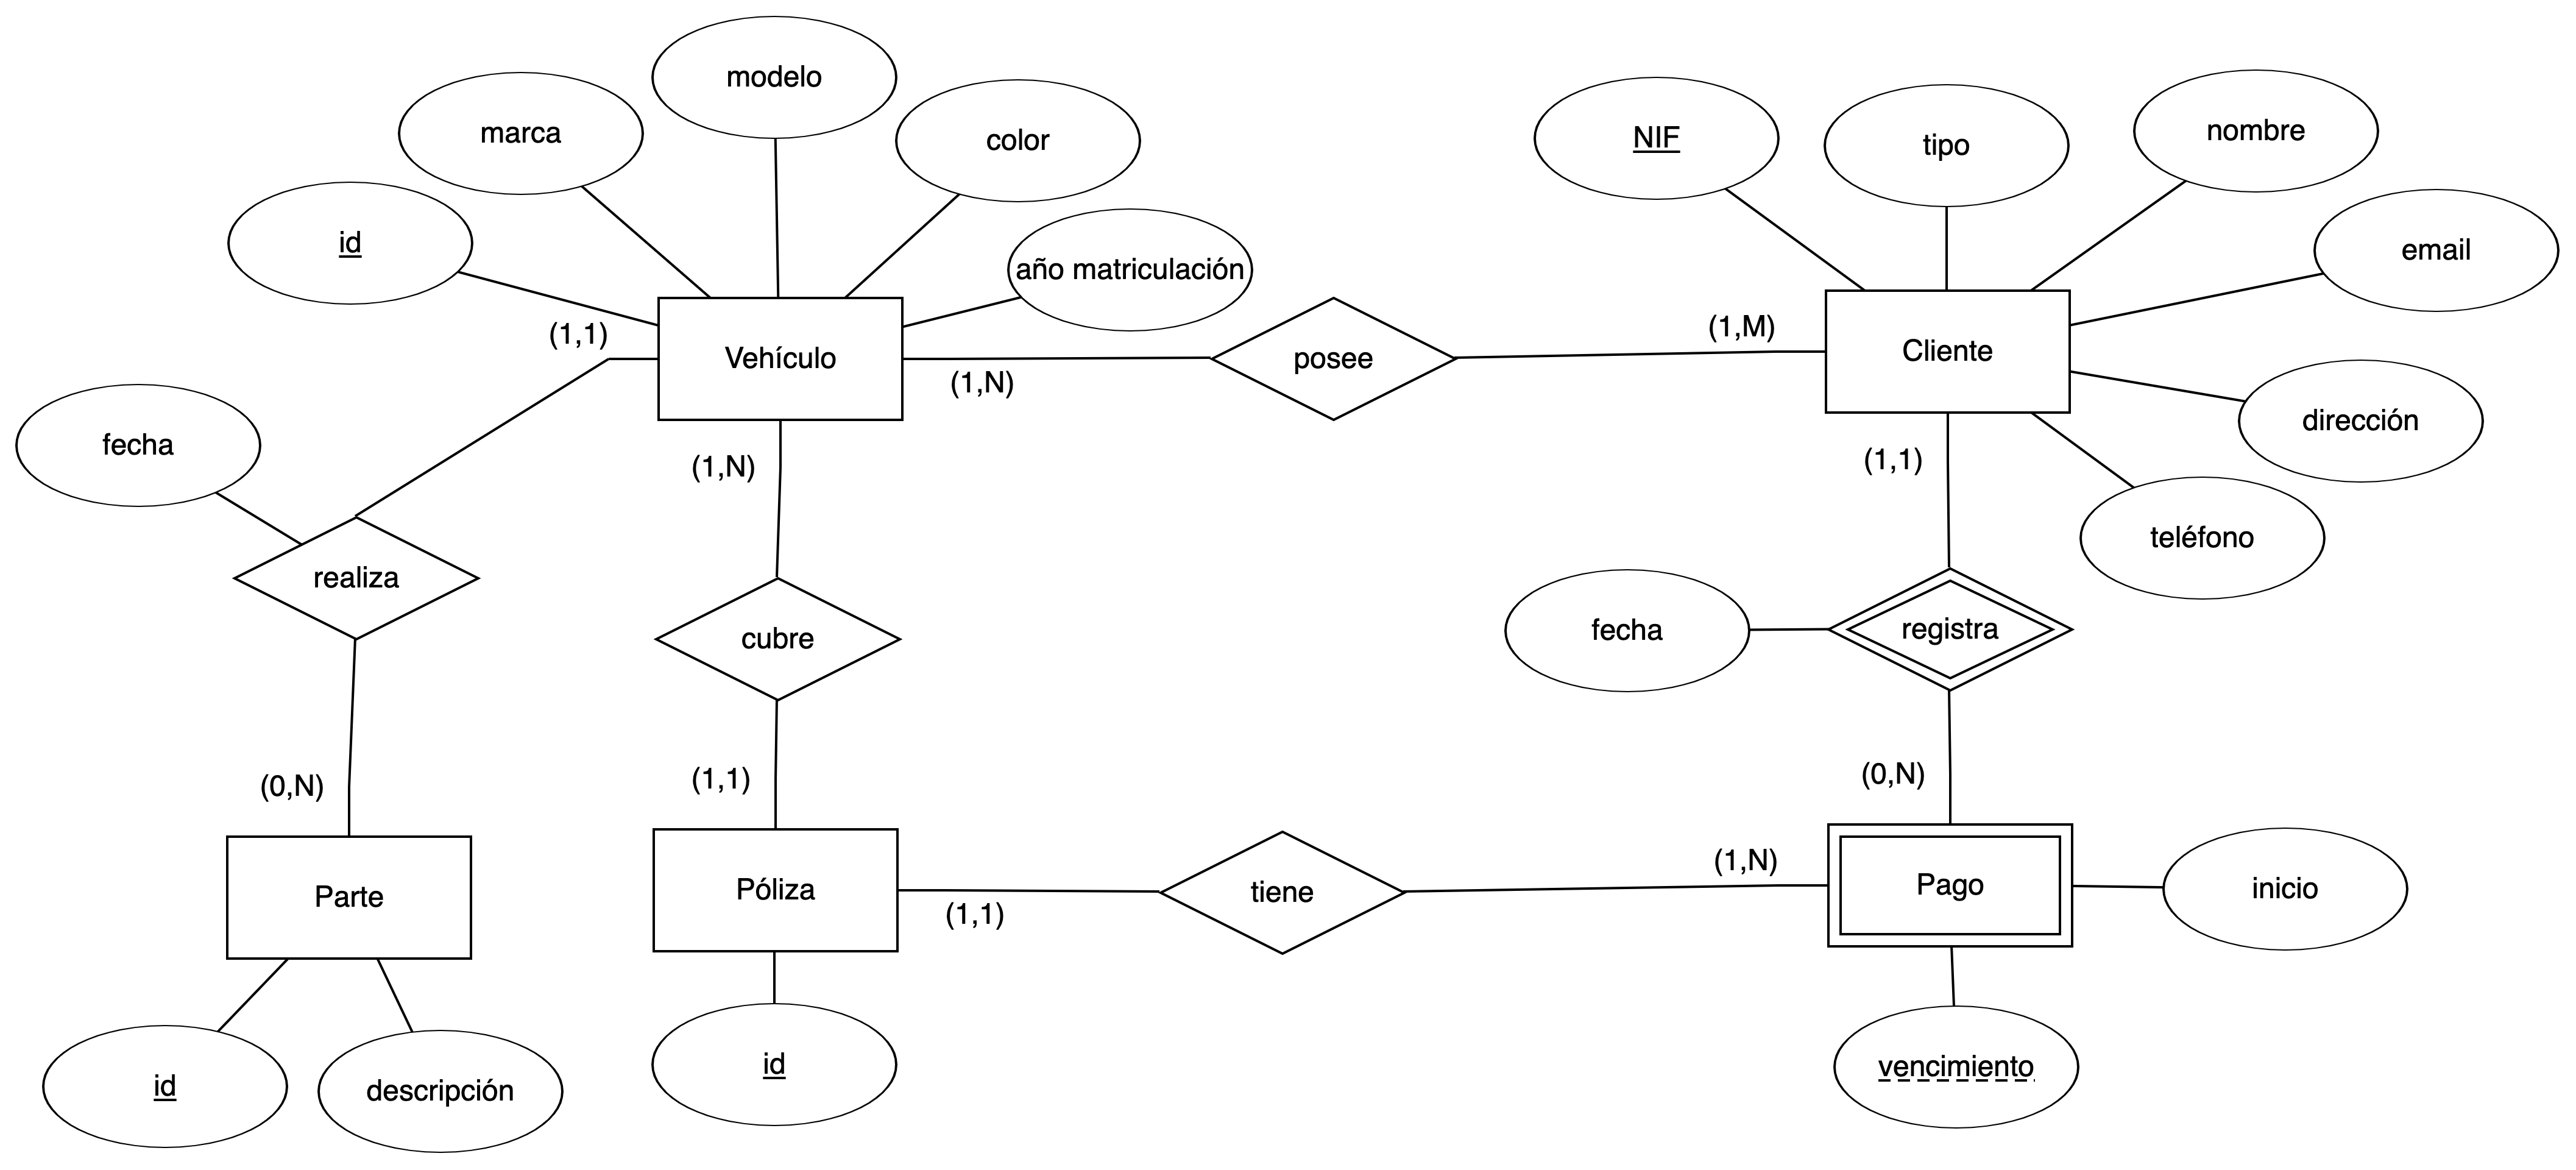
\includegraphics[width=\textwidth]{figs/ejercicio-1}
\end{figure}

\section{Paquetería}
\begin{figure}[H]
    \centering
    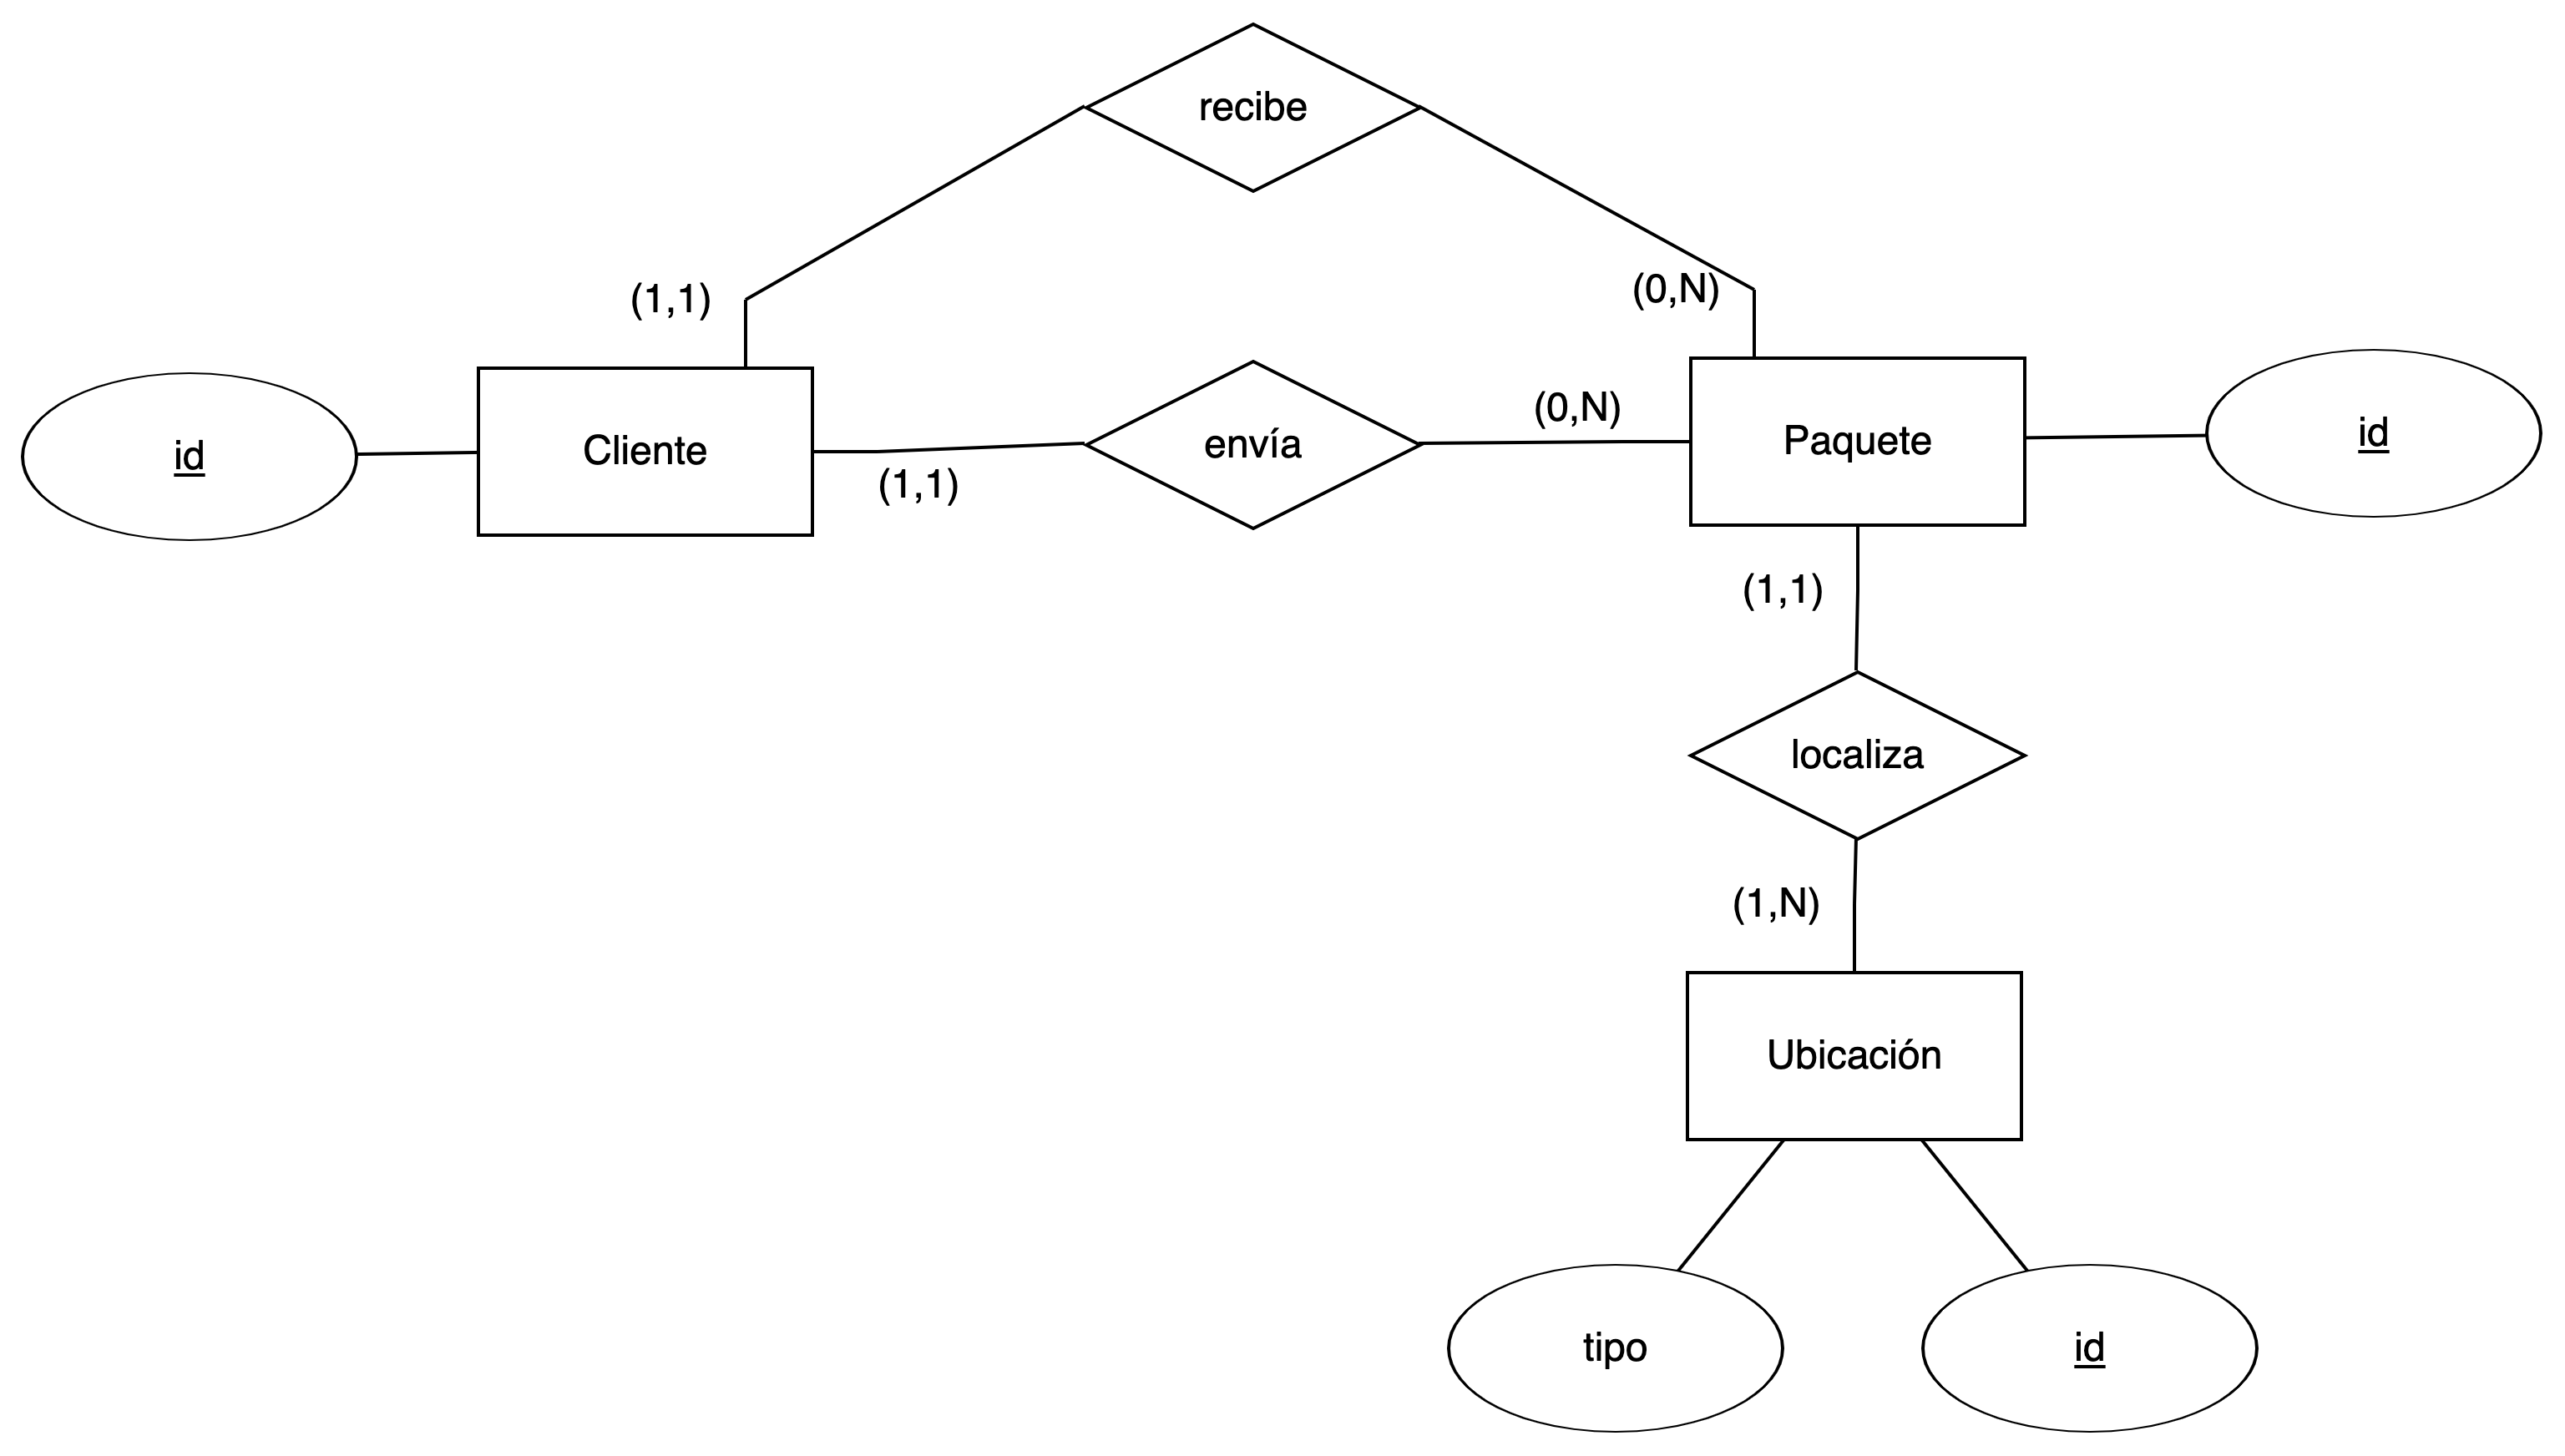
\includegraphics[width=\textwidth]{figs/ejercicio-2}
\end{figure}

\section{Tienda de mascotas}
\begin{figure}[H]
    \centering
    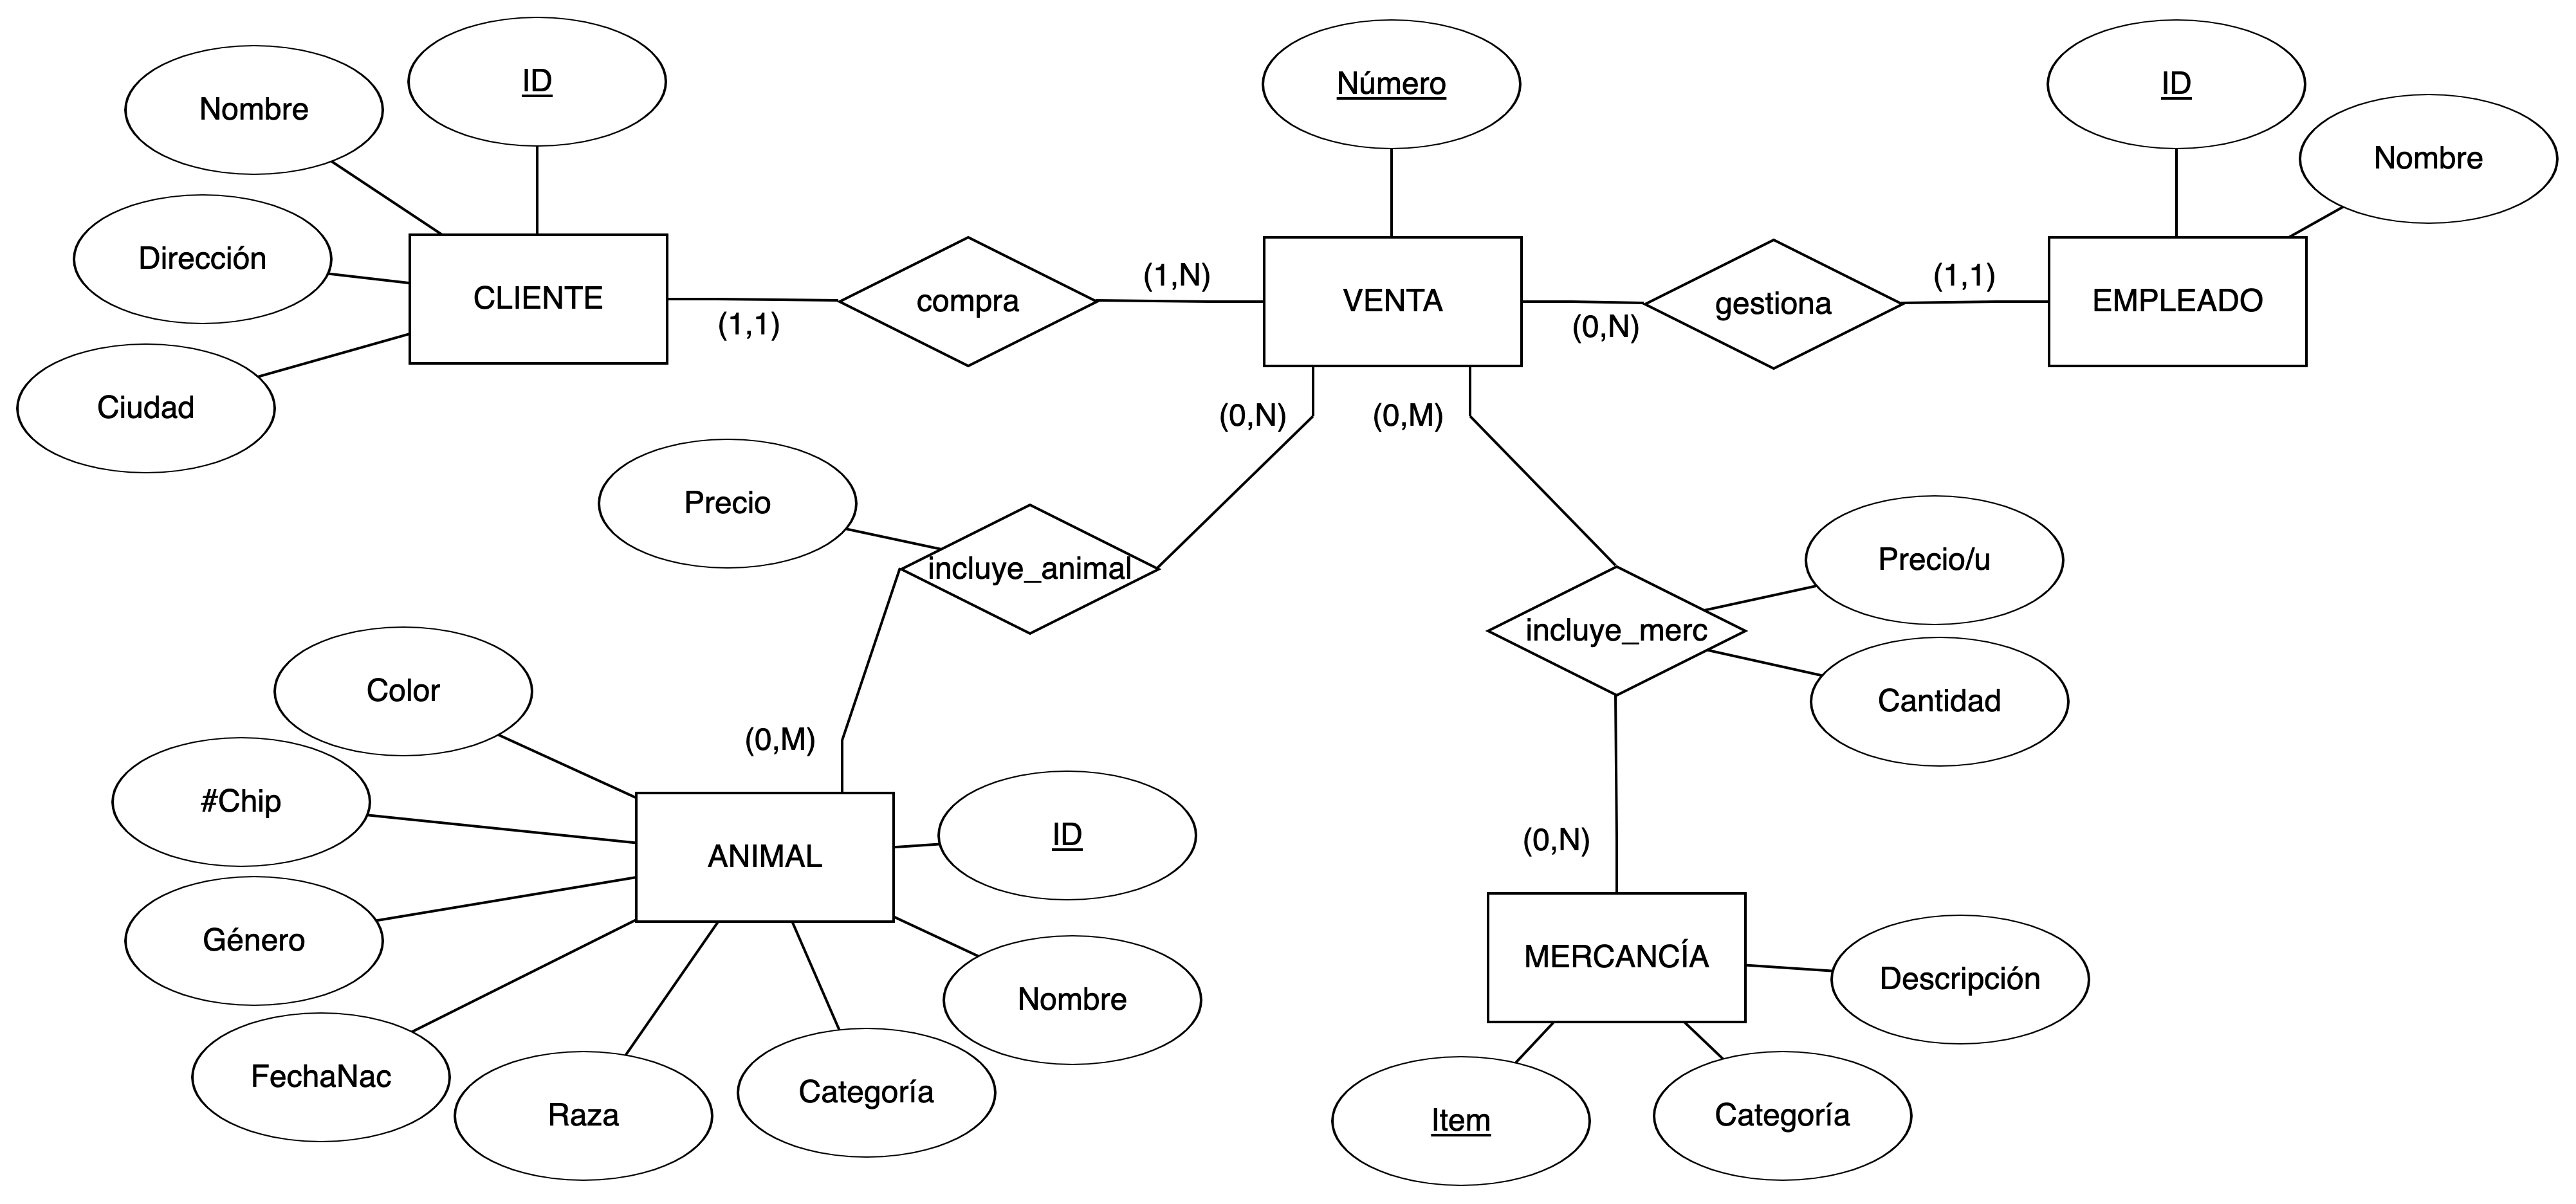
\includegraphics[width=\textwidth]{figs/ejercicio-3}
\end{figure}

\section{Hospital}
\begin{figure}[H]
    \centering
    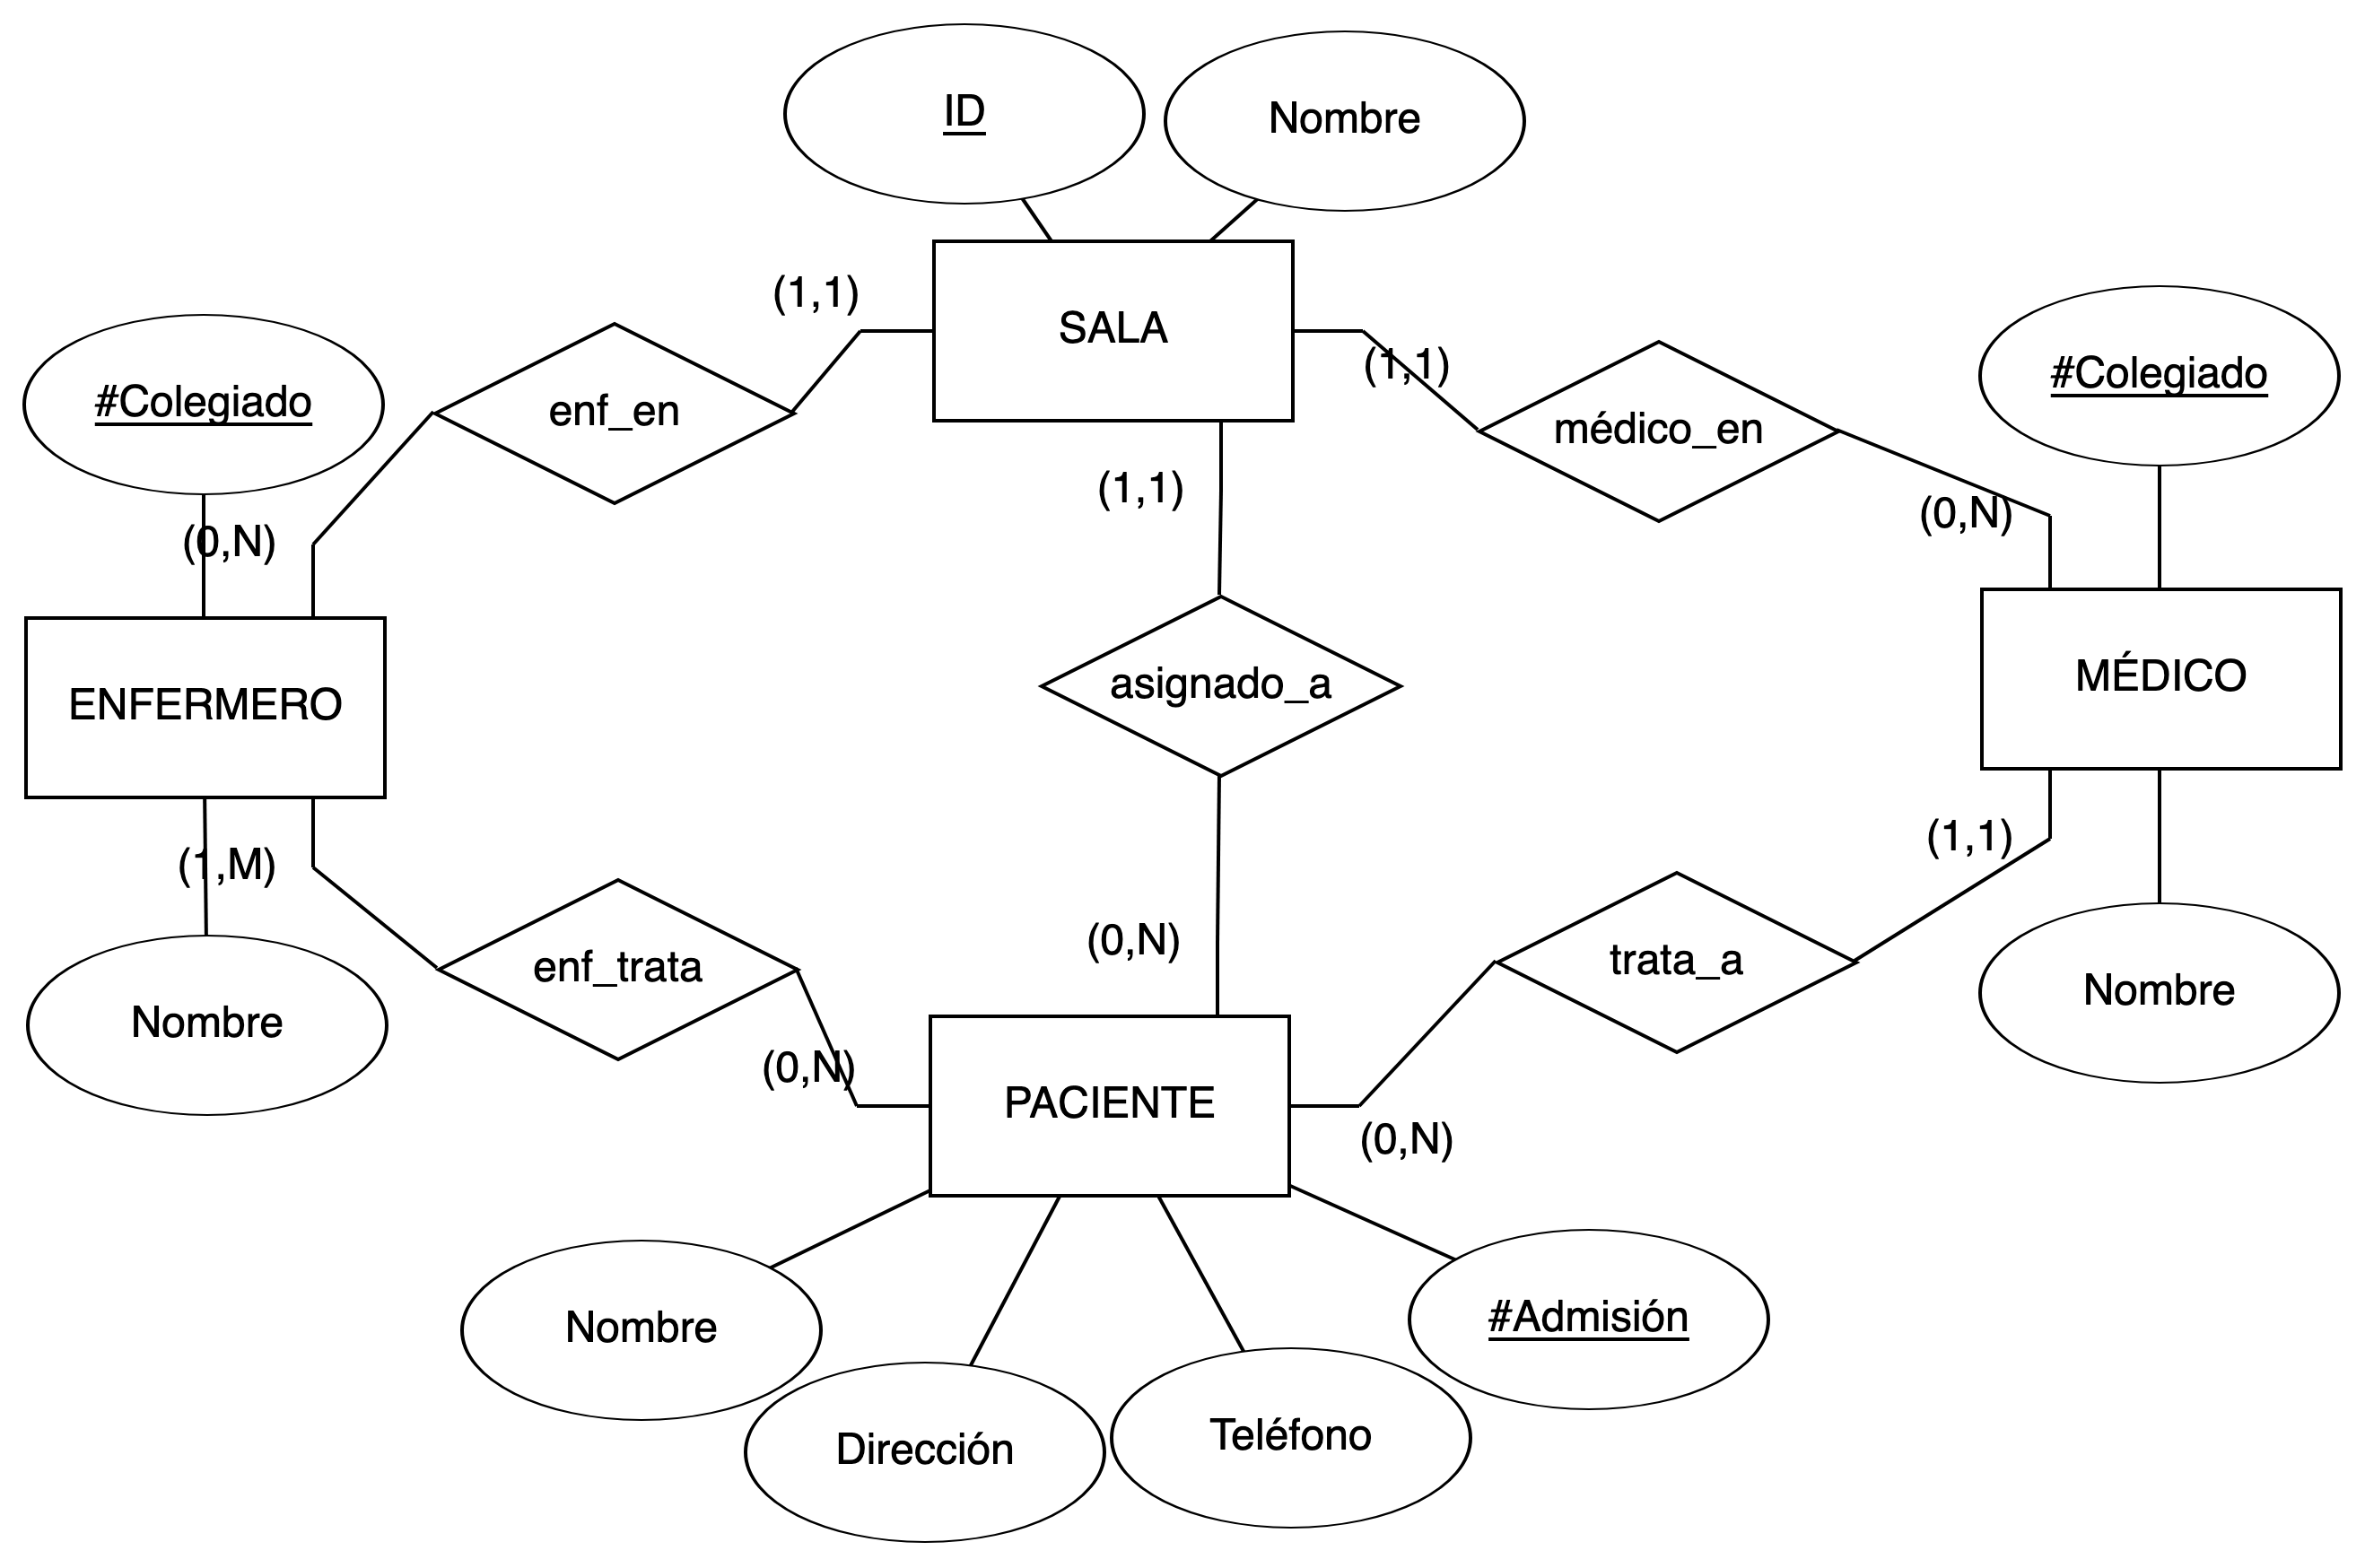
\includegraphics[width=\textwidth]{figs/ejercicio-4}
\end{figure}

\section{Permisos de circulación}
\begin{figure}[H]
    \centering
    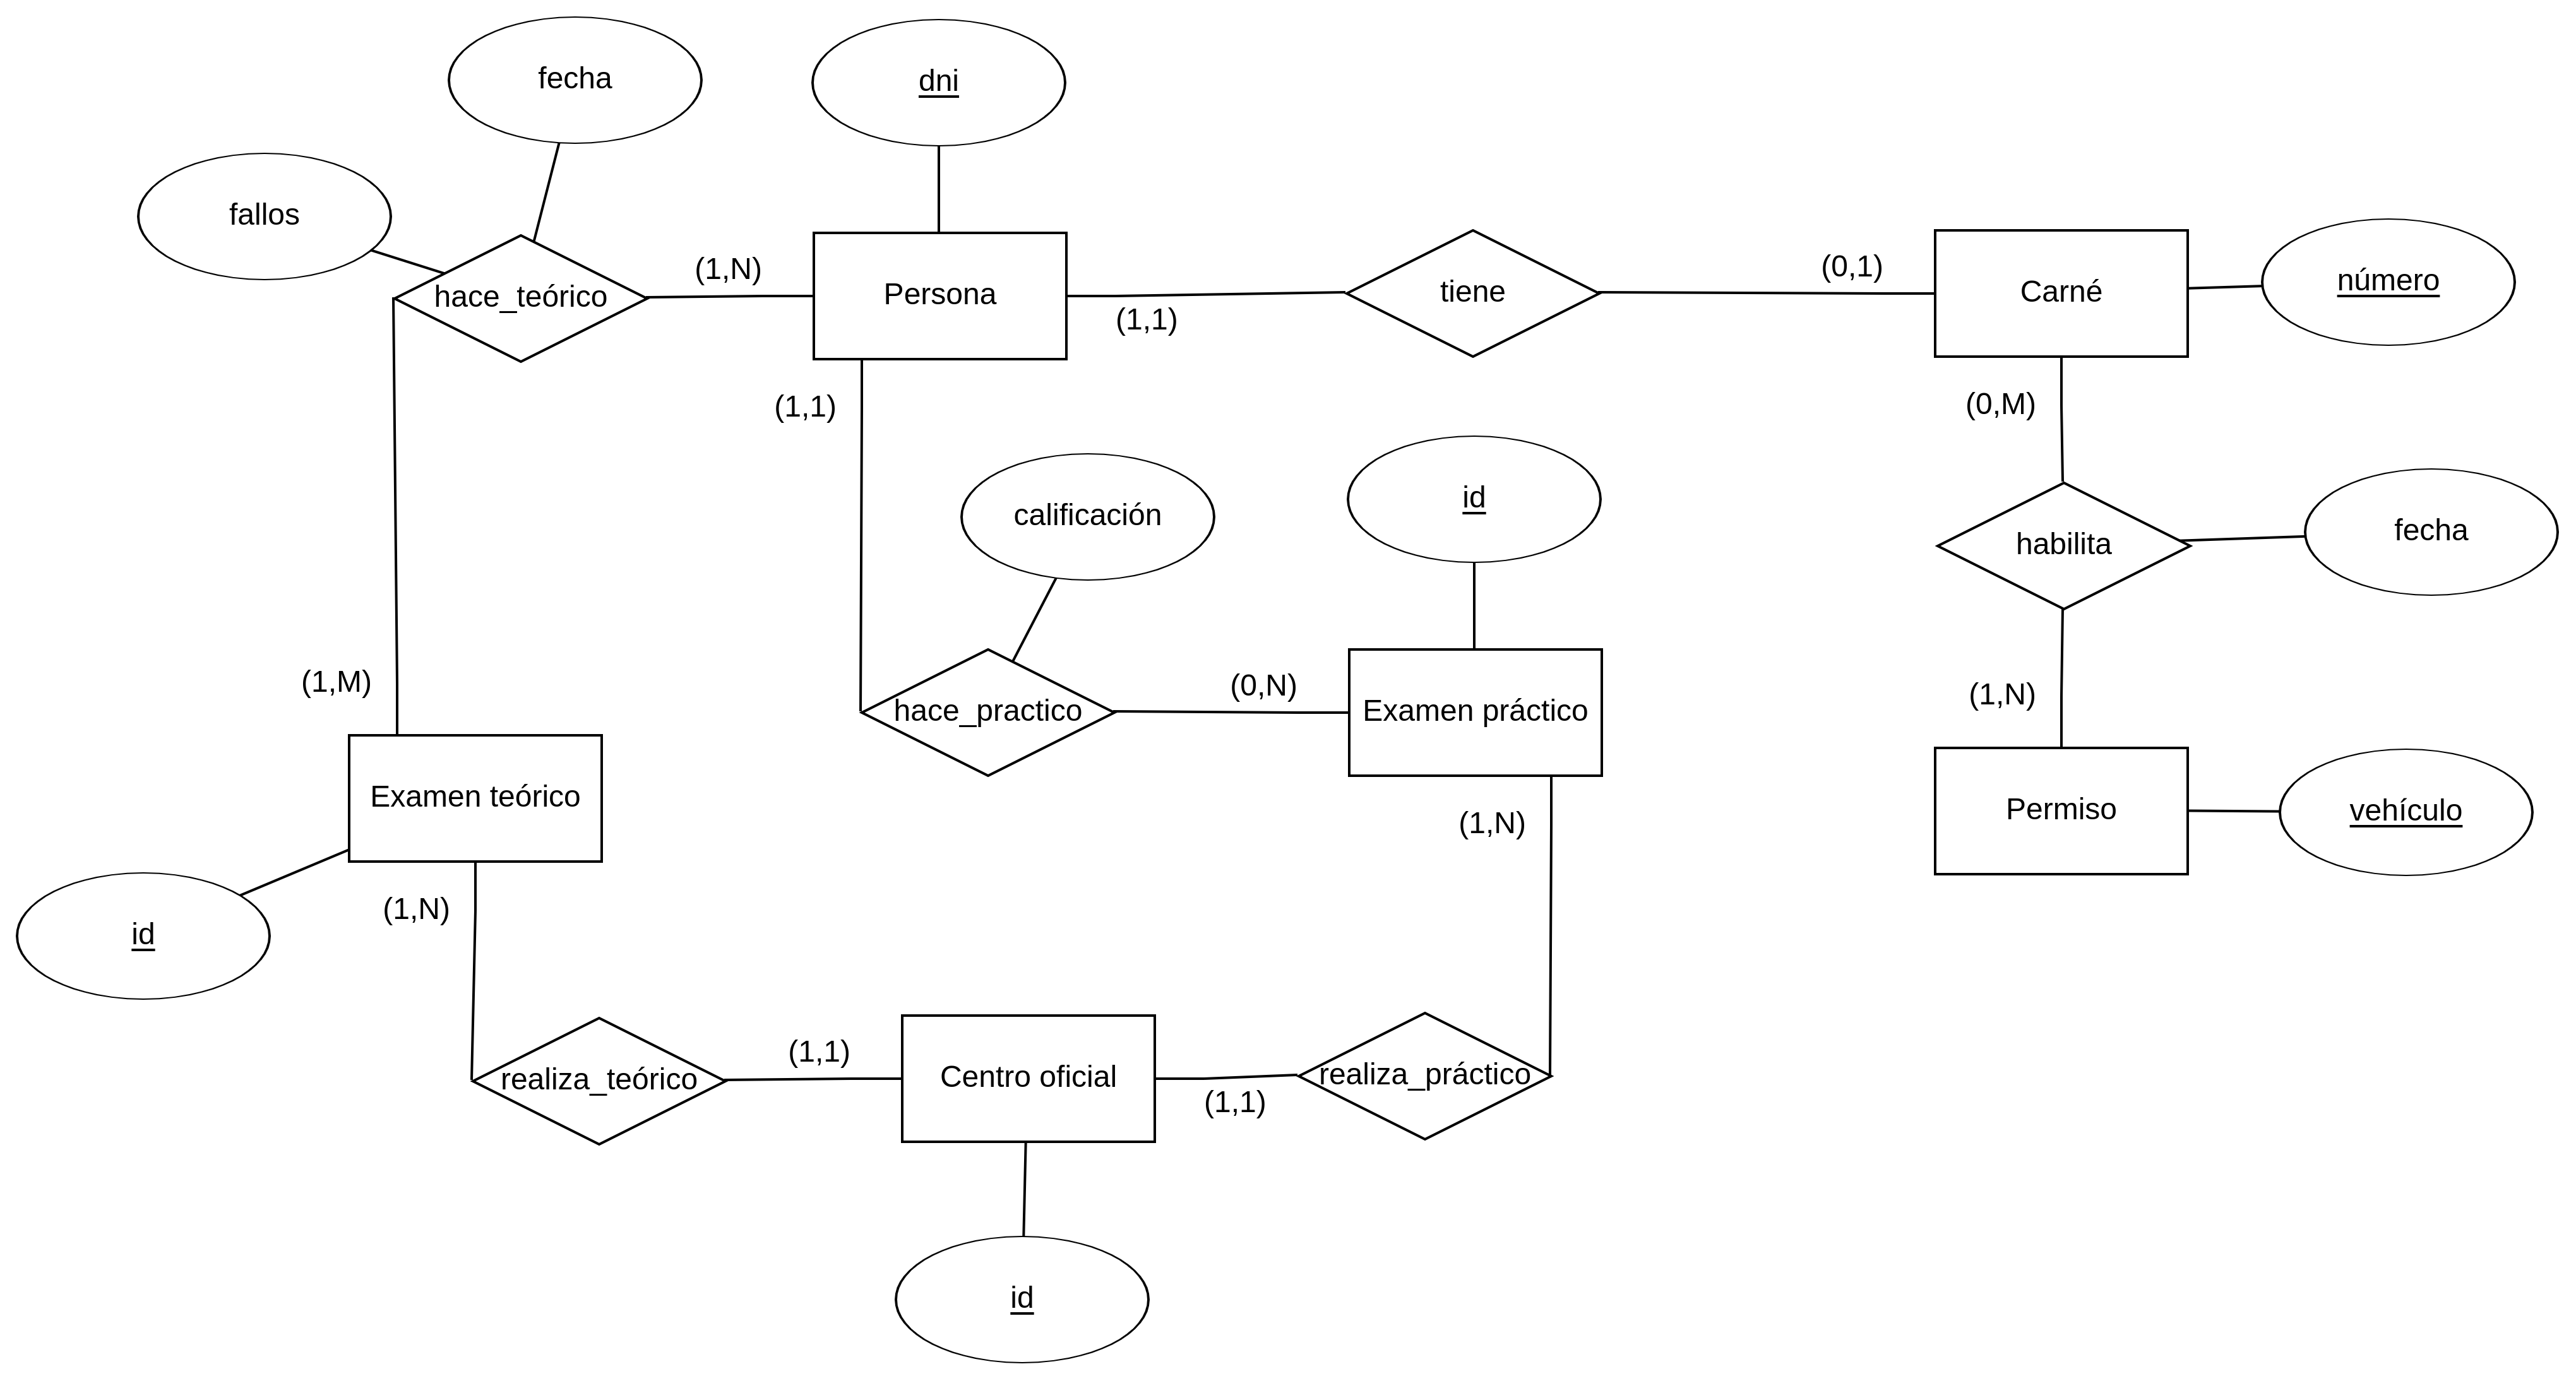
\includegraphics[width=\textwidth]{figs/ejercicio-5}
\end{figure}

\section{Galería de arte}
\begin{figure}[H]
    \centering
    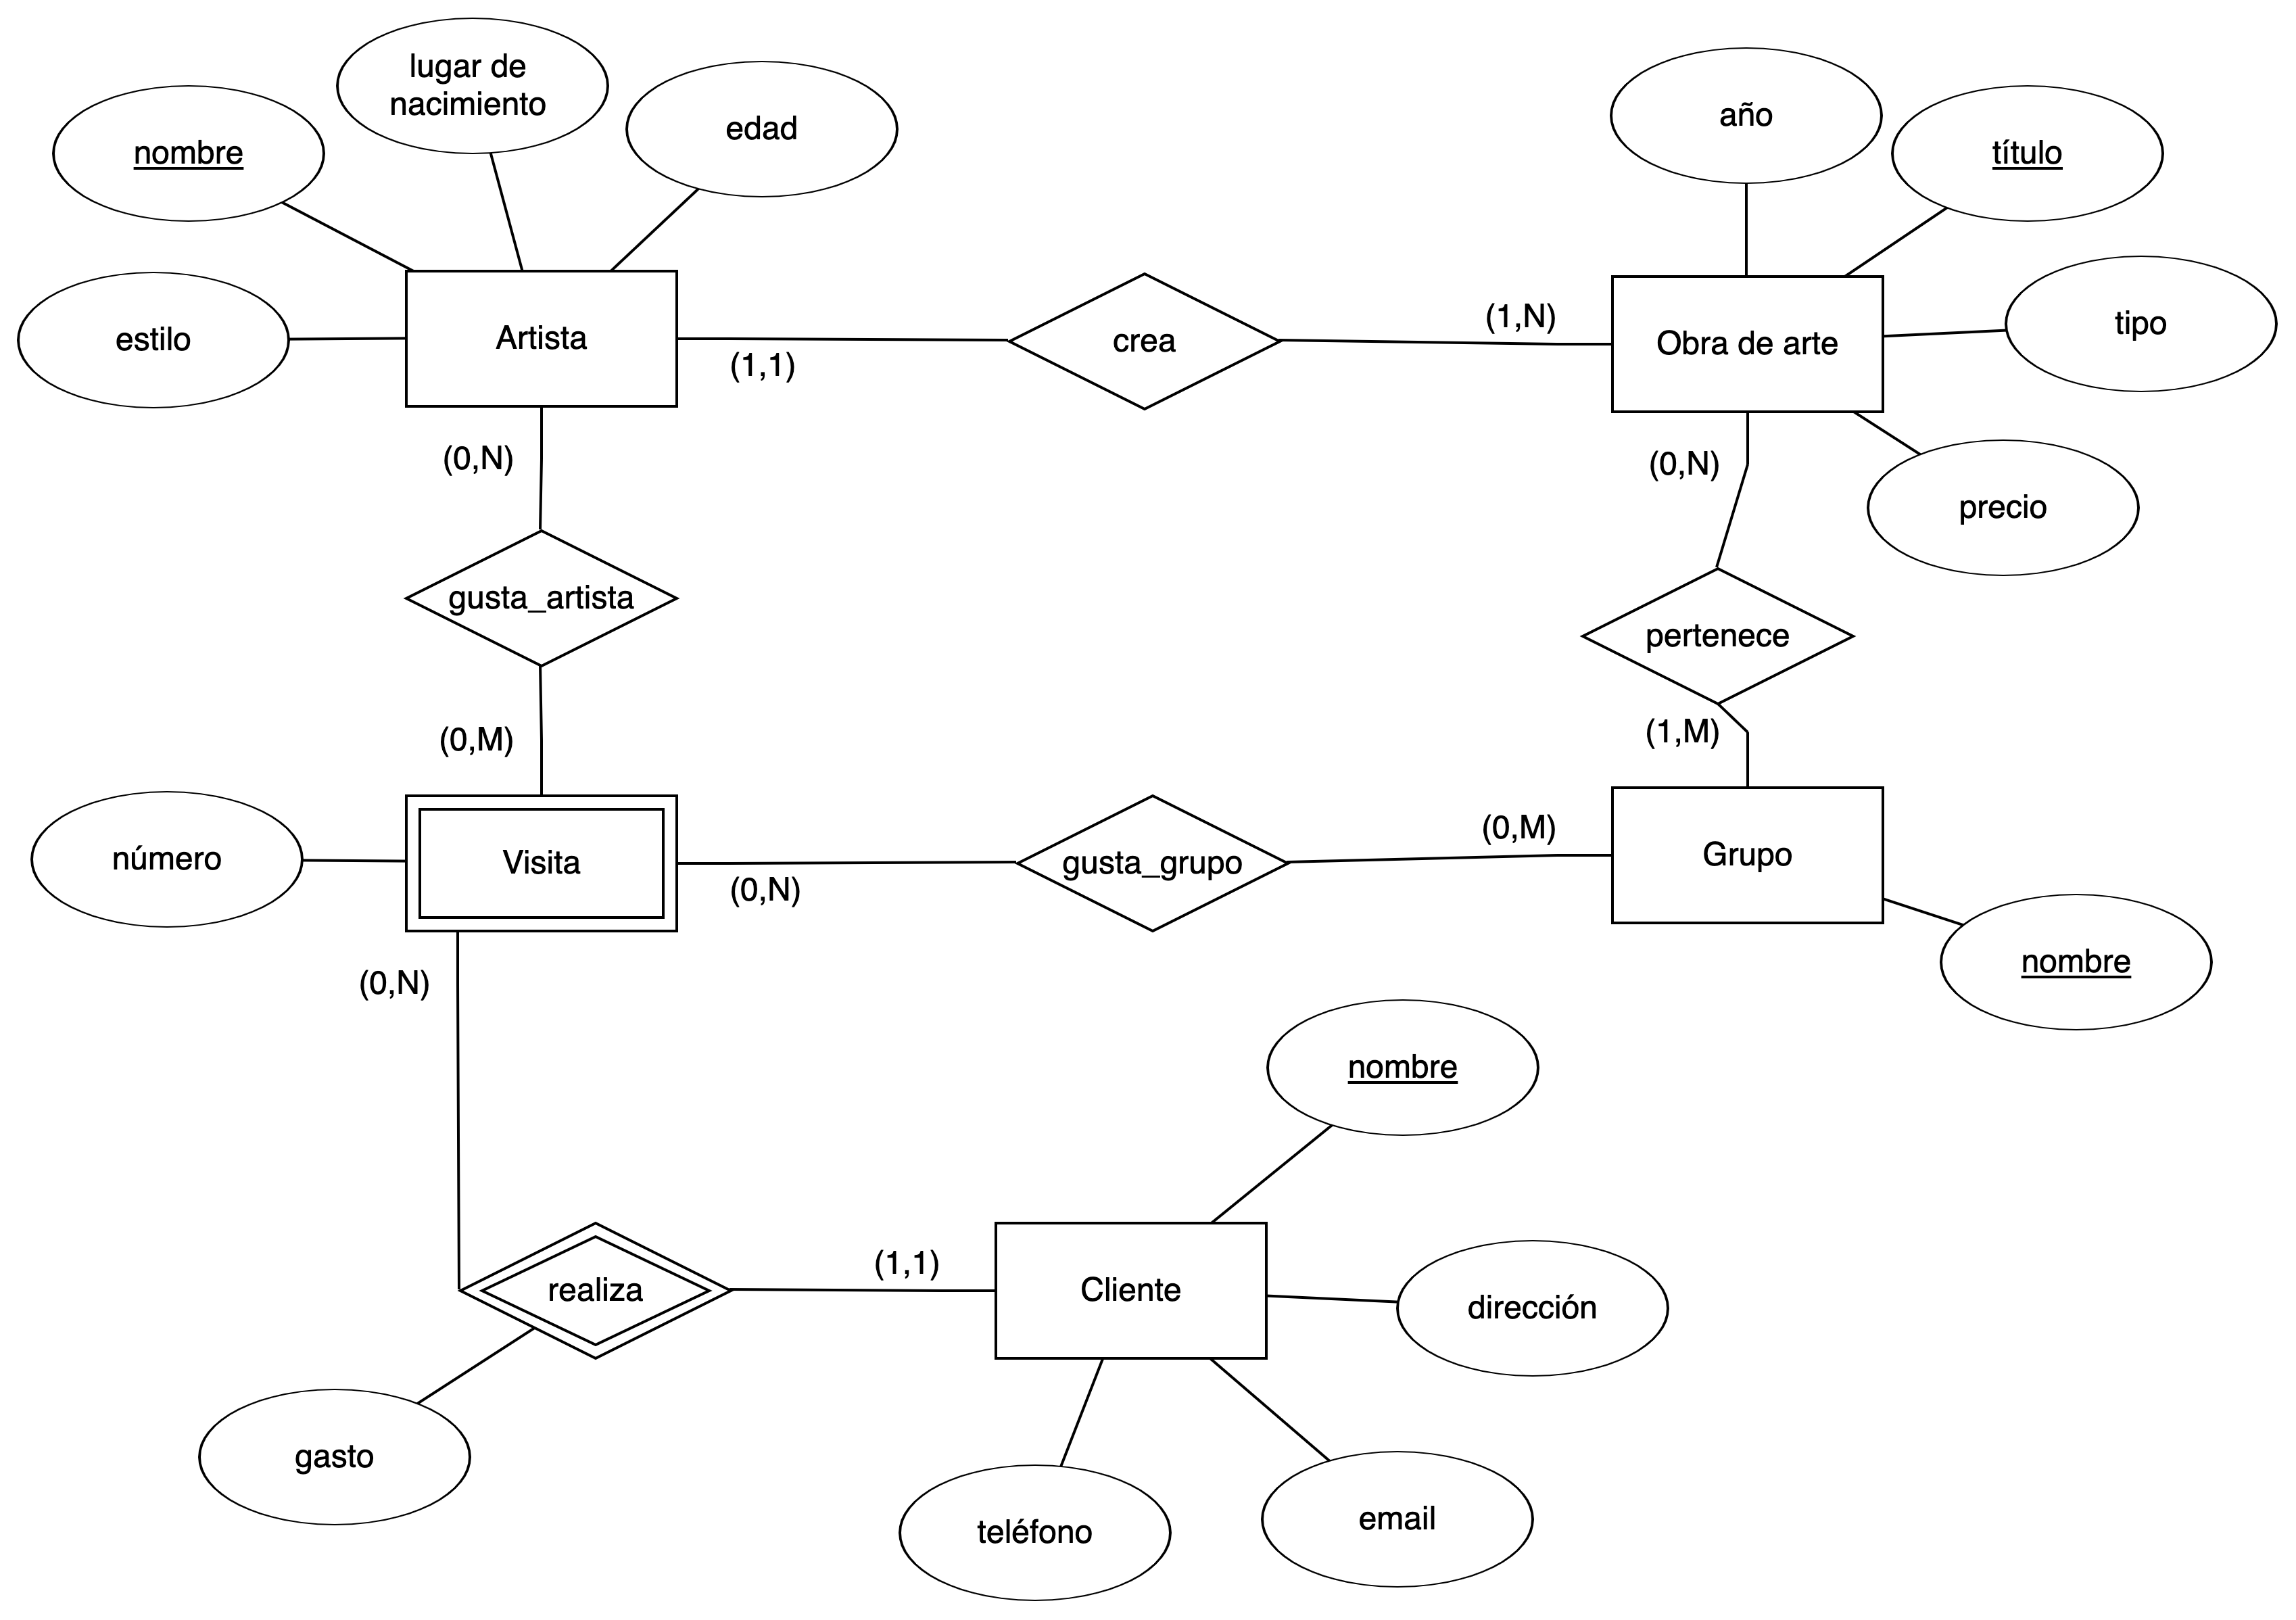
\includegraphics[width=\textwidth]{figs/ejercicio-6}
\end{figure}

\section{Gimnasio}
\begin{figure}[H]
    \centering
    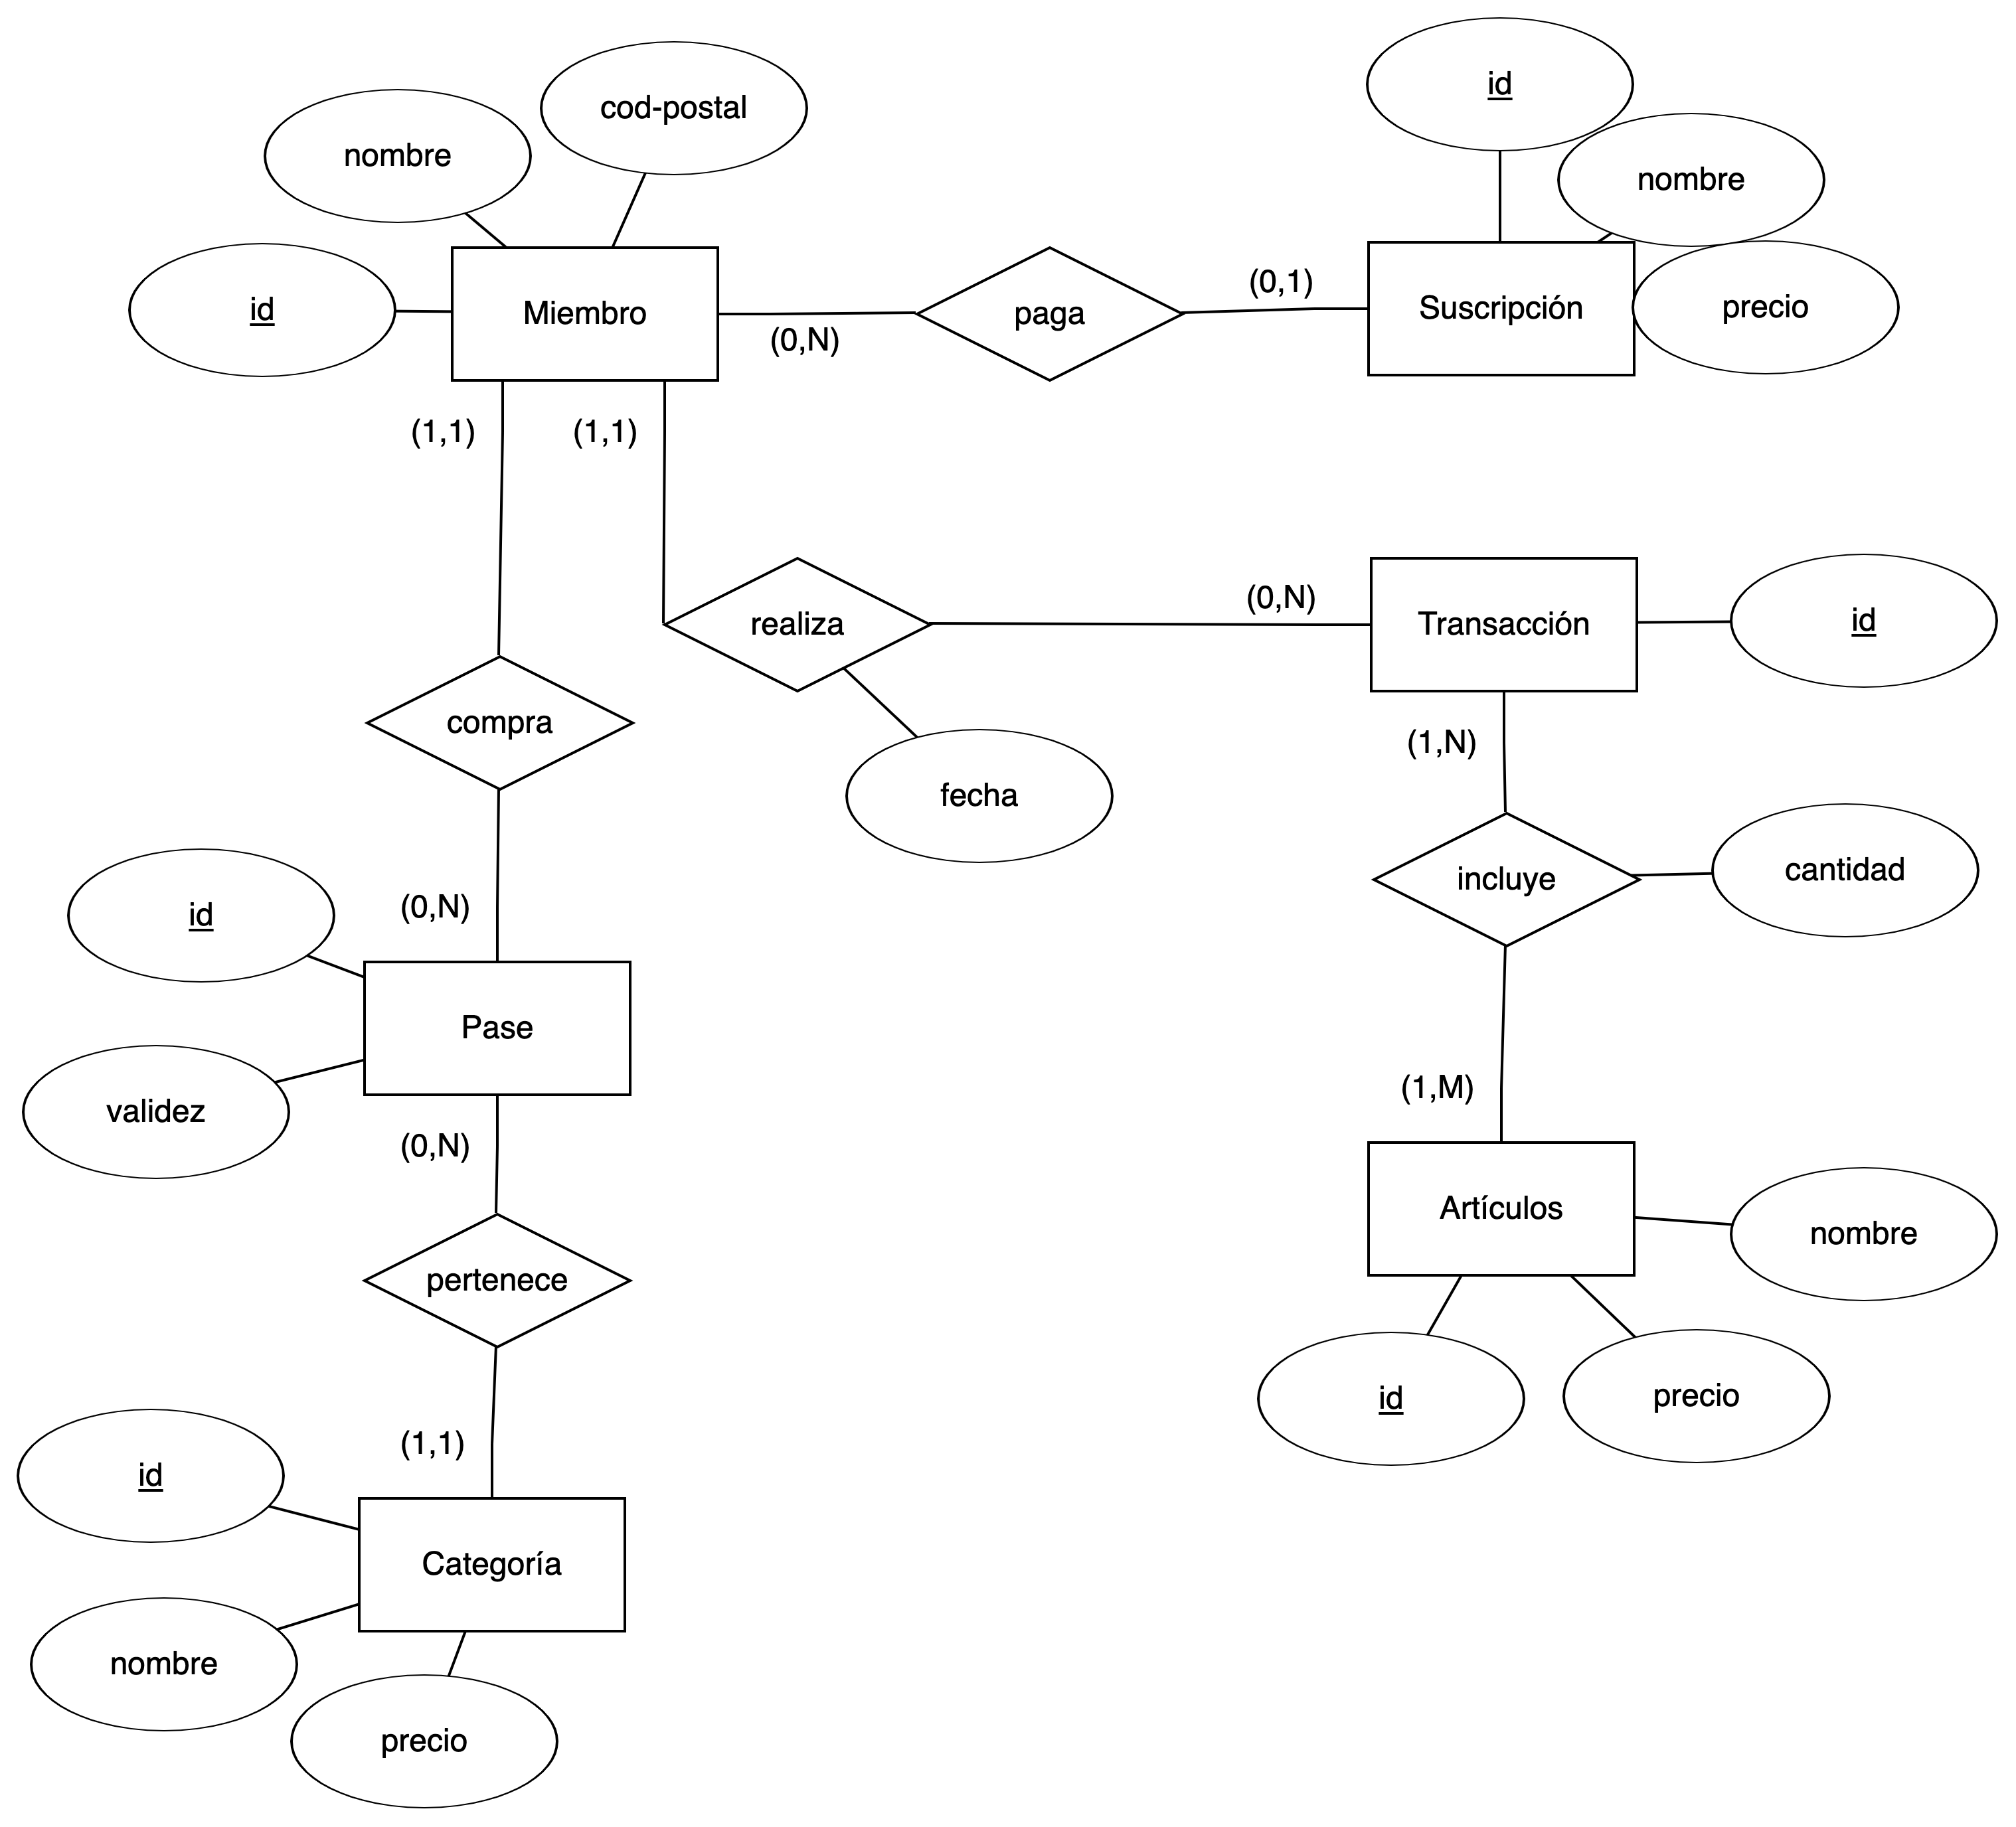
\includegraphics[width=\textwidth]{figs/ejercicio-7}
\end{figure}

\section{Alquiler de coches}
\begin{figure}[H]
    \centering
    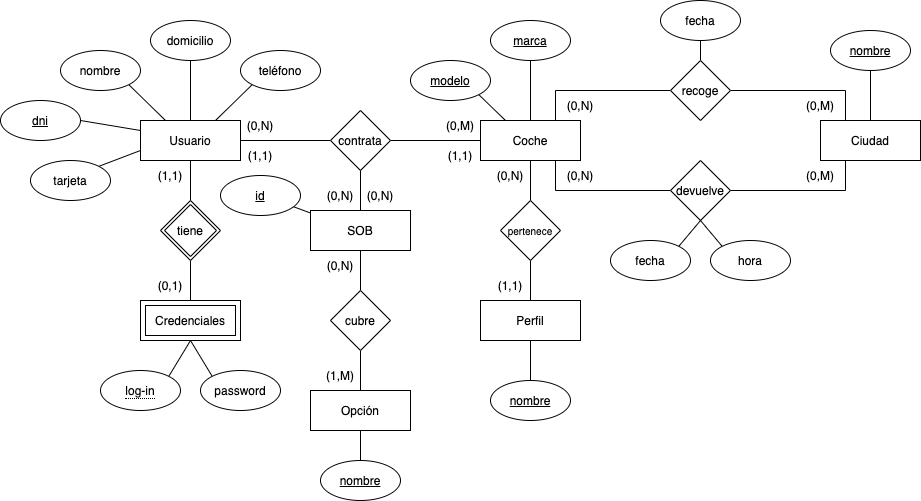
\includegraphics[width=\textwidth]{figs/ejercicio-8}
\end{figure}

\section{Censo de la Unión Europea}
\begin{figure}[H]
    \centering
    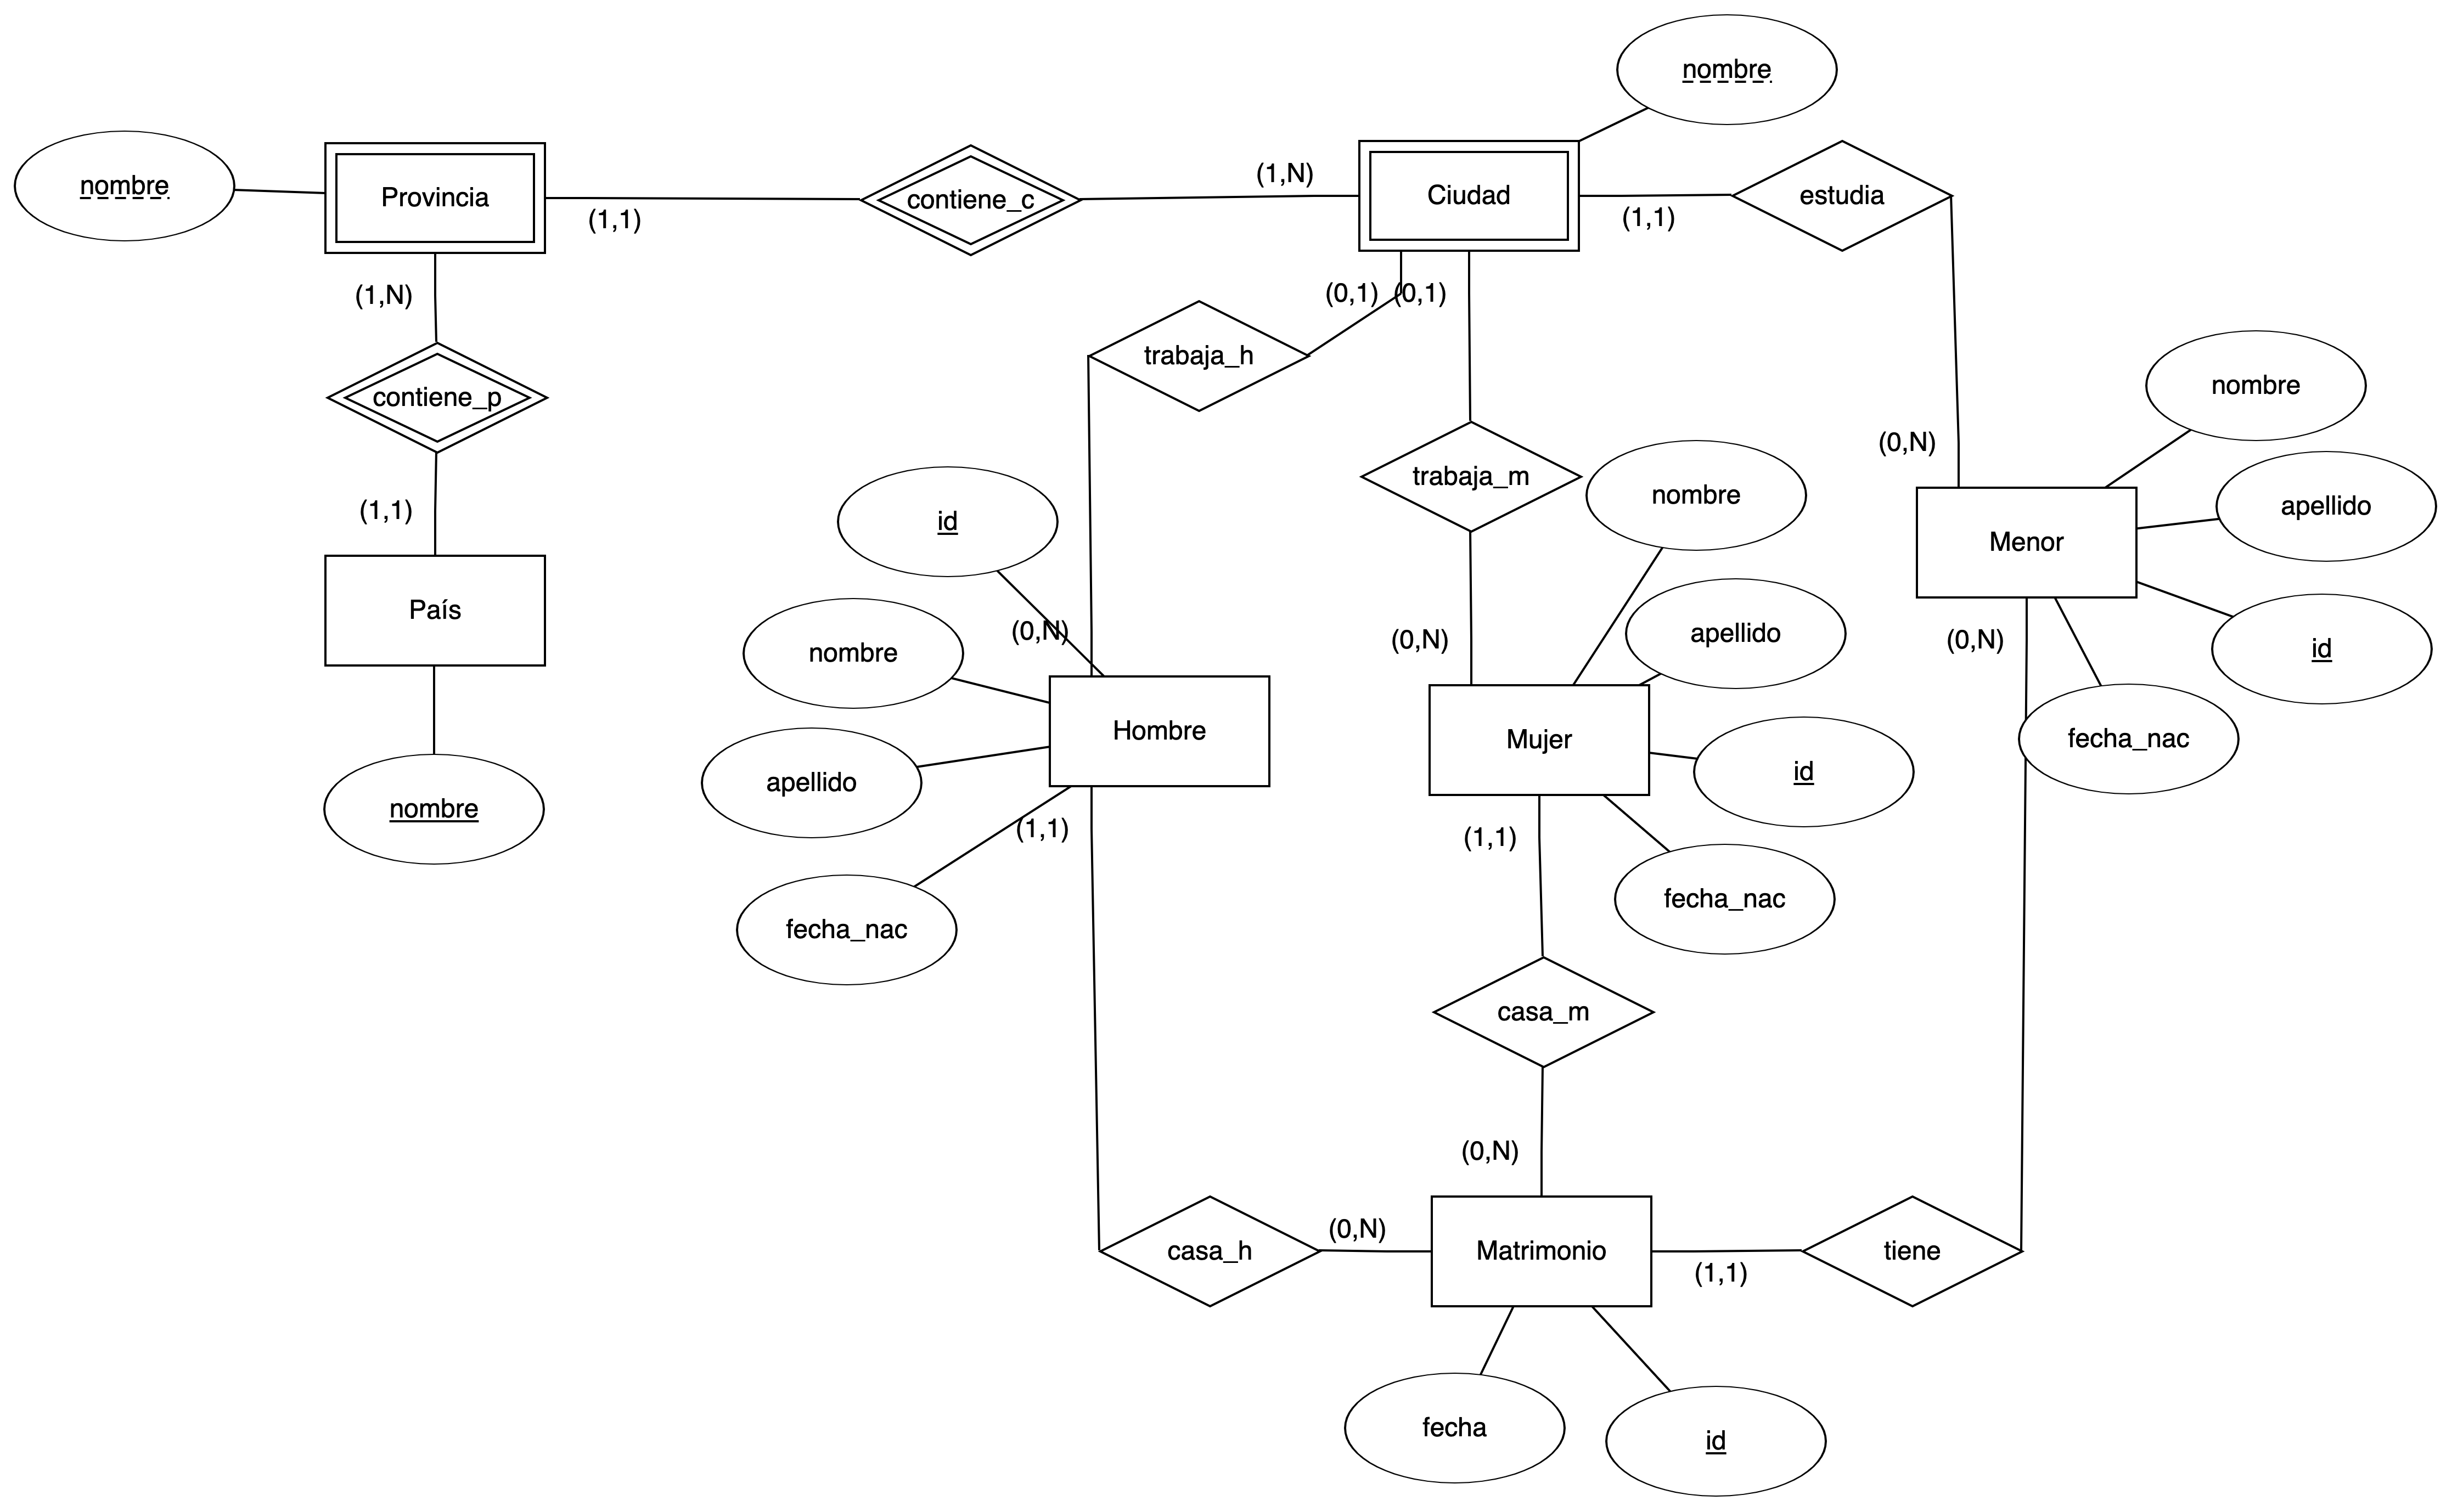
\includegraphics[width=\textwidth]{figs/ejercicio-9}
\end{figure}

\section{Subastas en línea}
\begin{figure}[H]
    \centering
    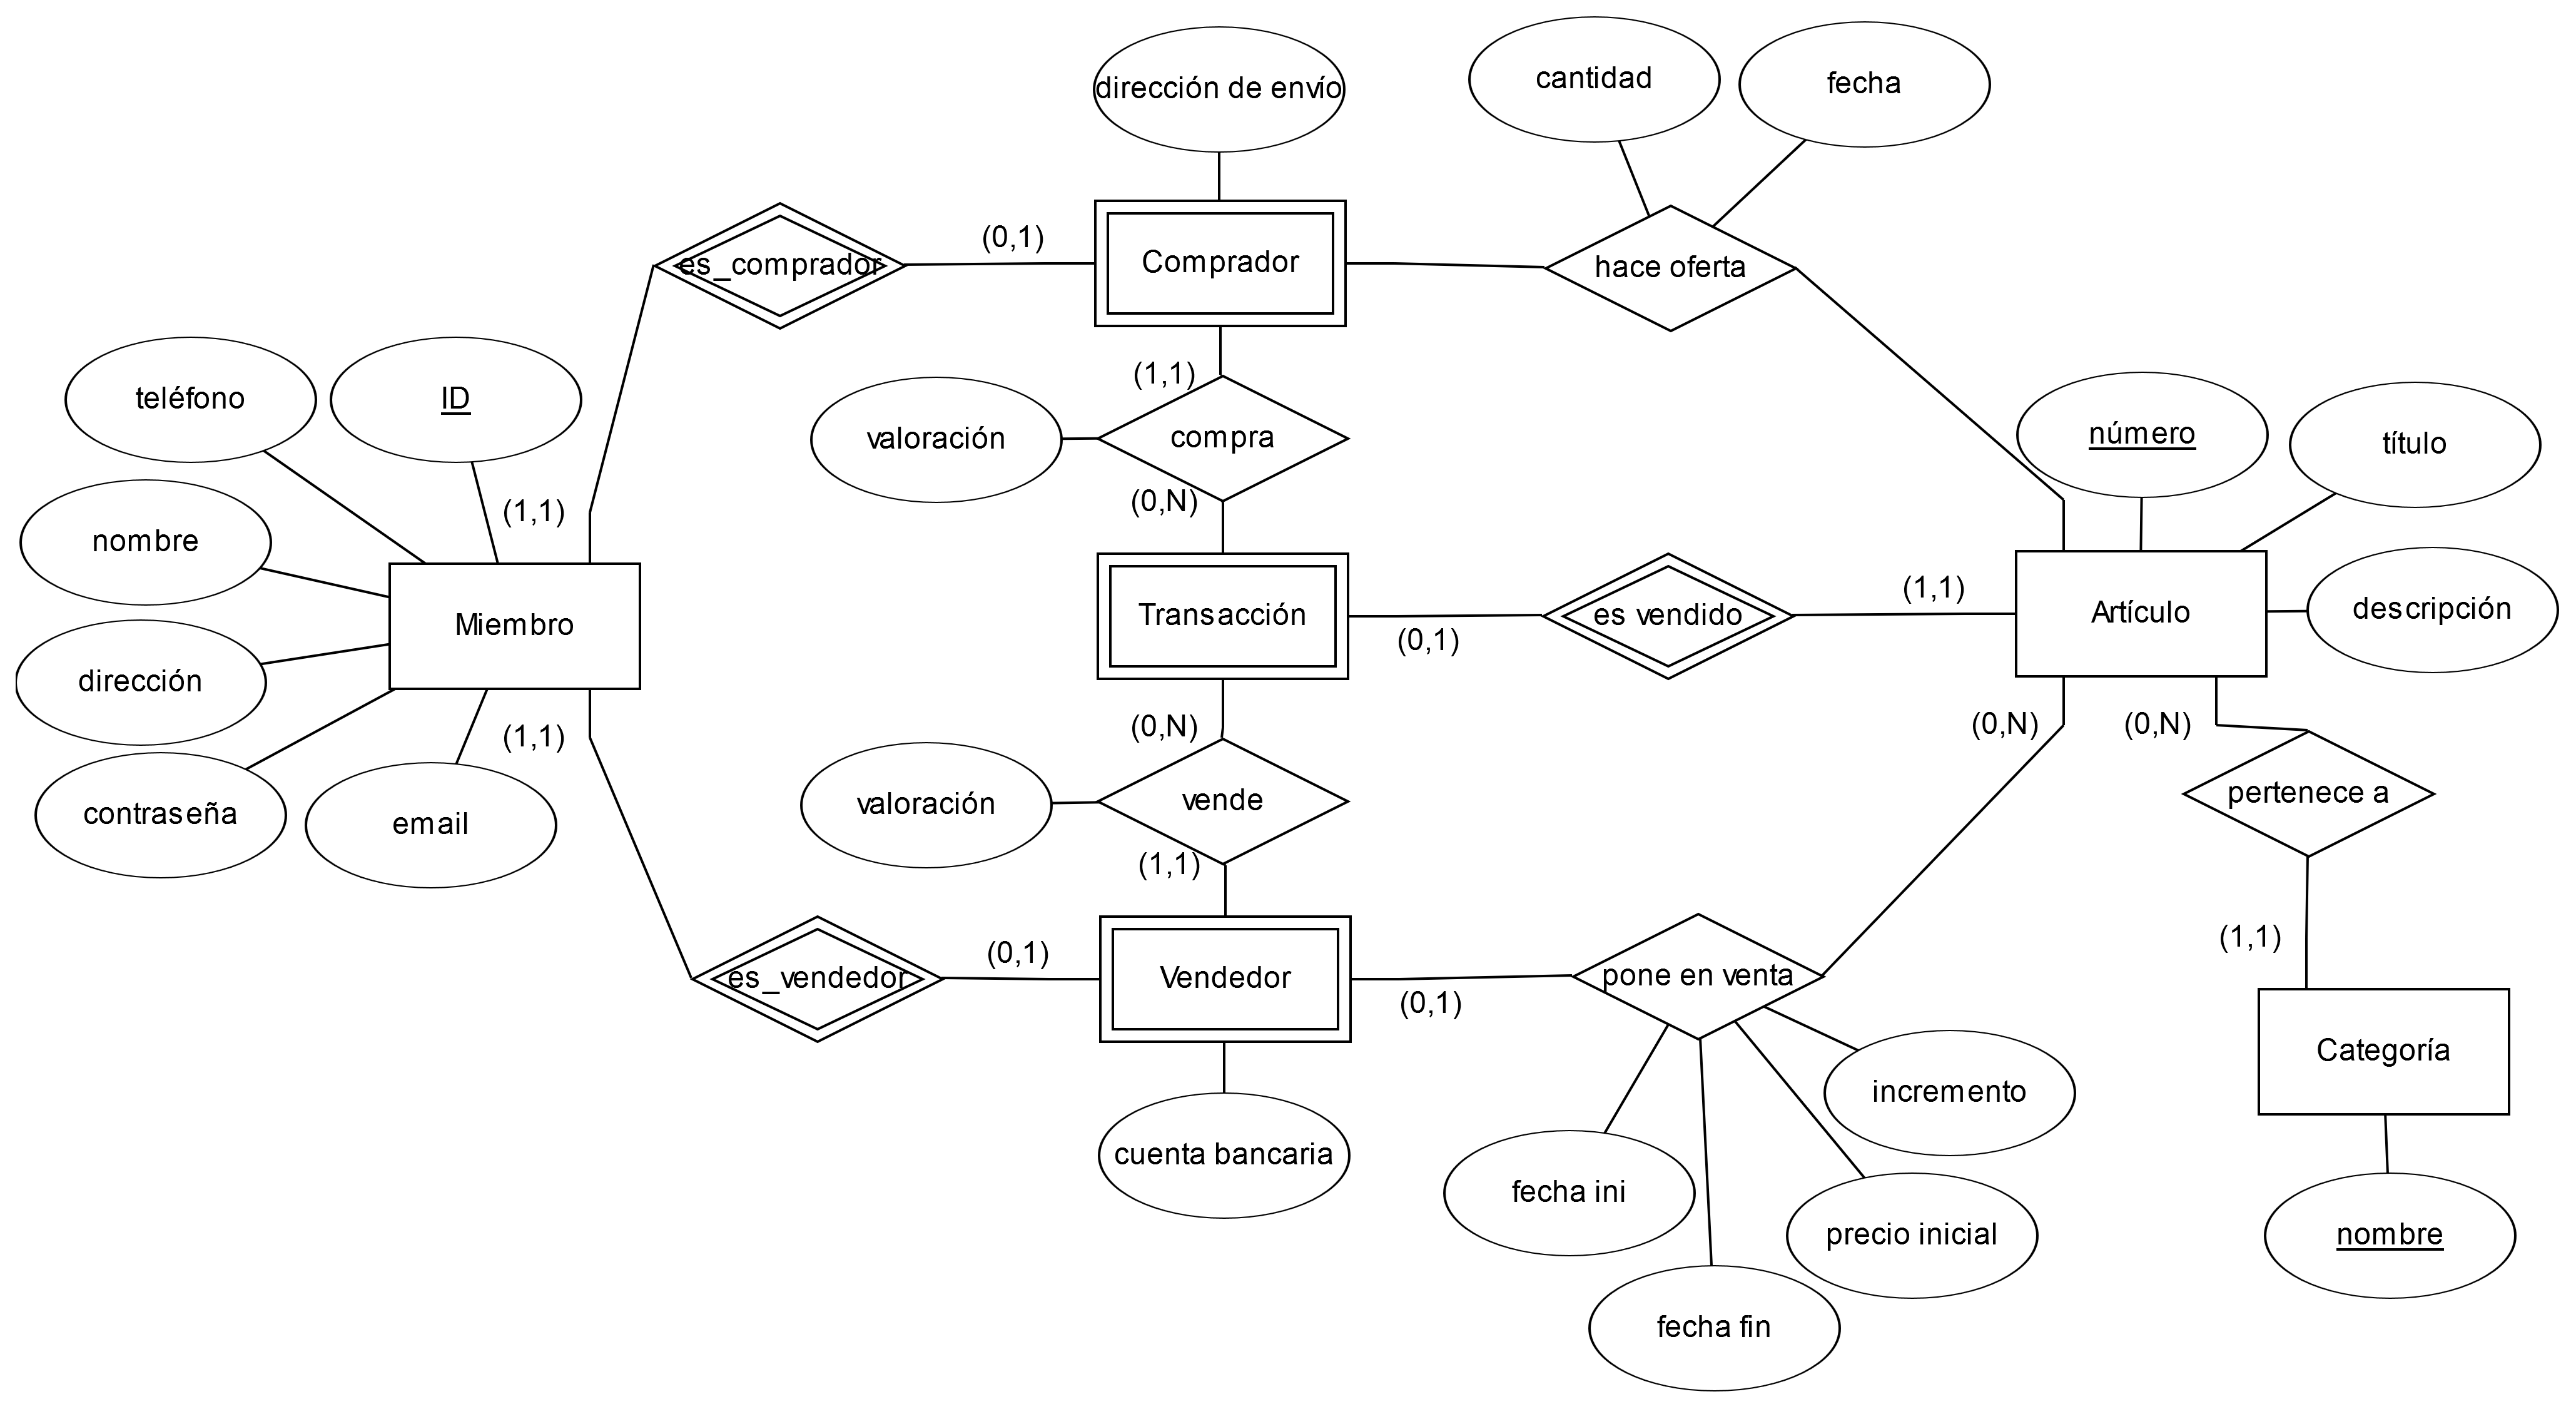
\includegraphics[width=\textwidth]{figs/ejercicio-10}
\end{figure}

\section{Cadena de restaurantes}
\begin{figure}[H]
    \centering
    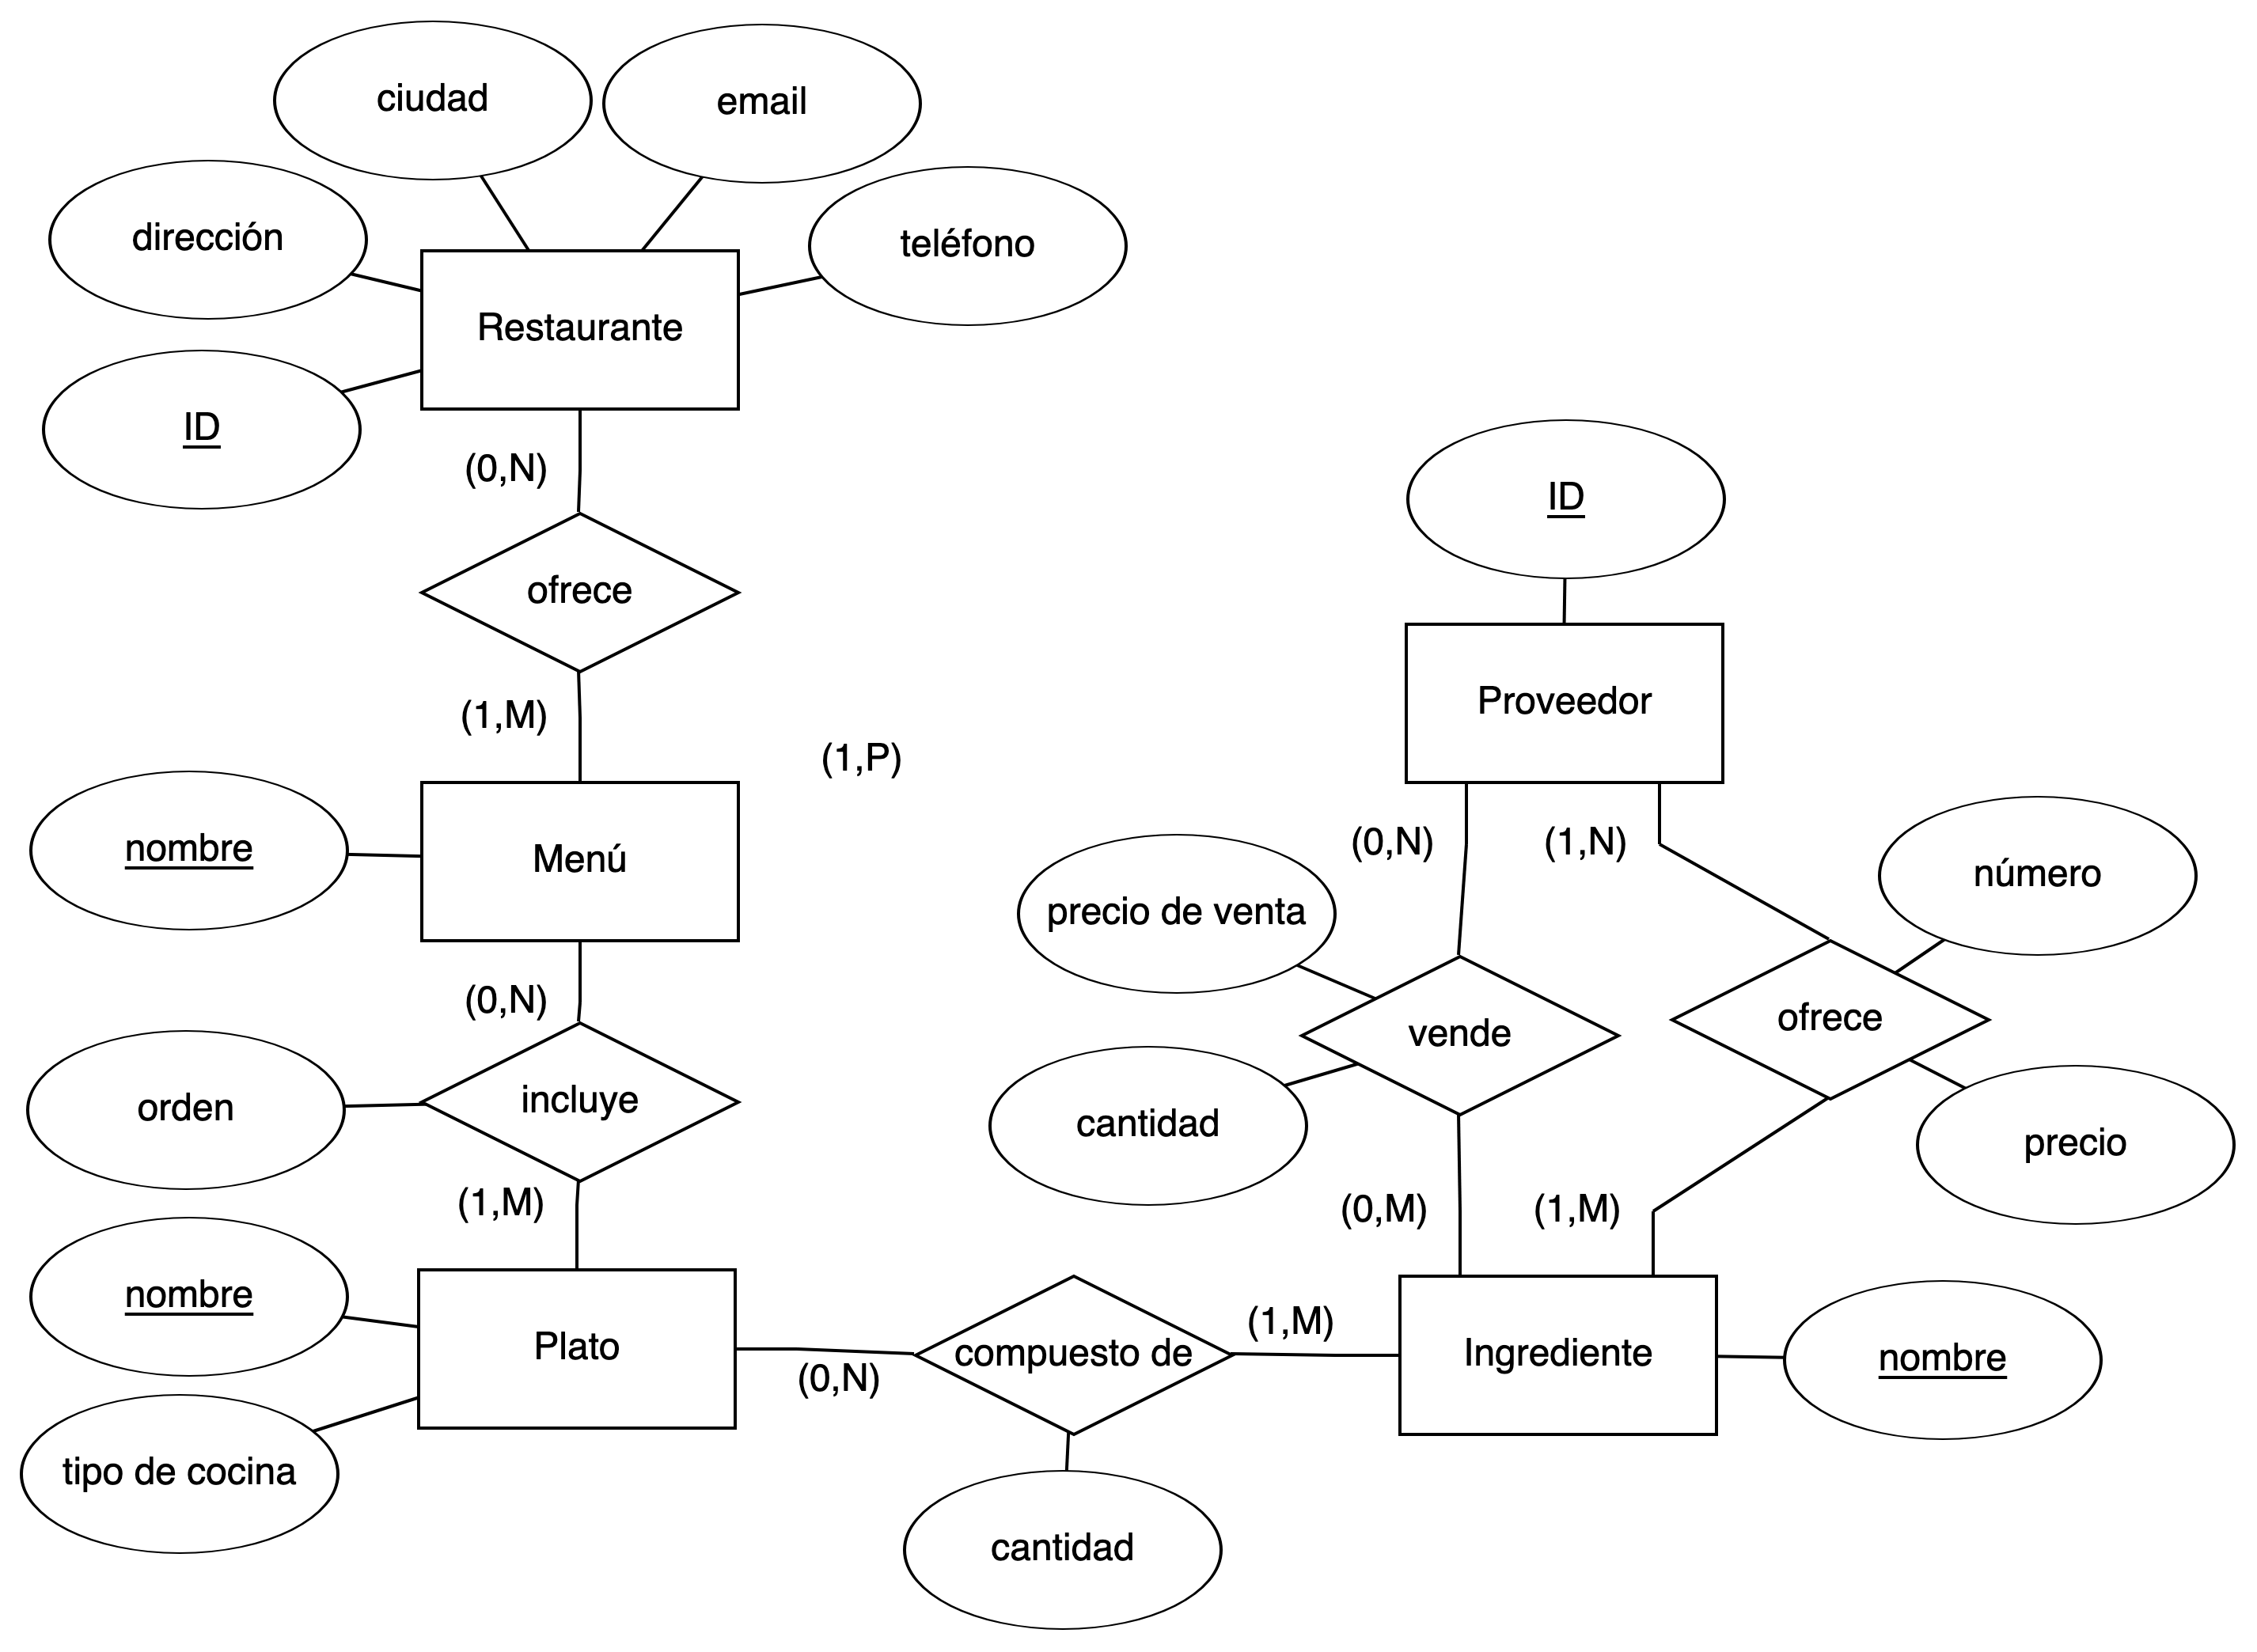
\includegraphics[width=\textwidth]{figs/ejercicio-11}
\end{figure}

\section{Exposición de pósteres}
\begin{figure}[H]
    \centering
    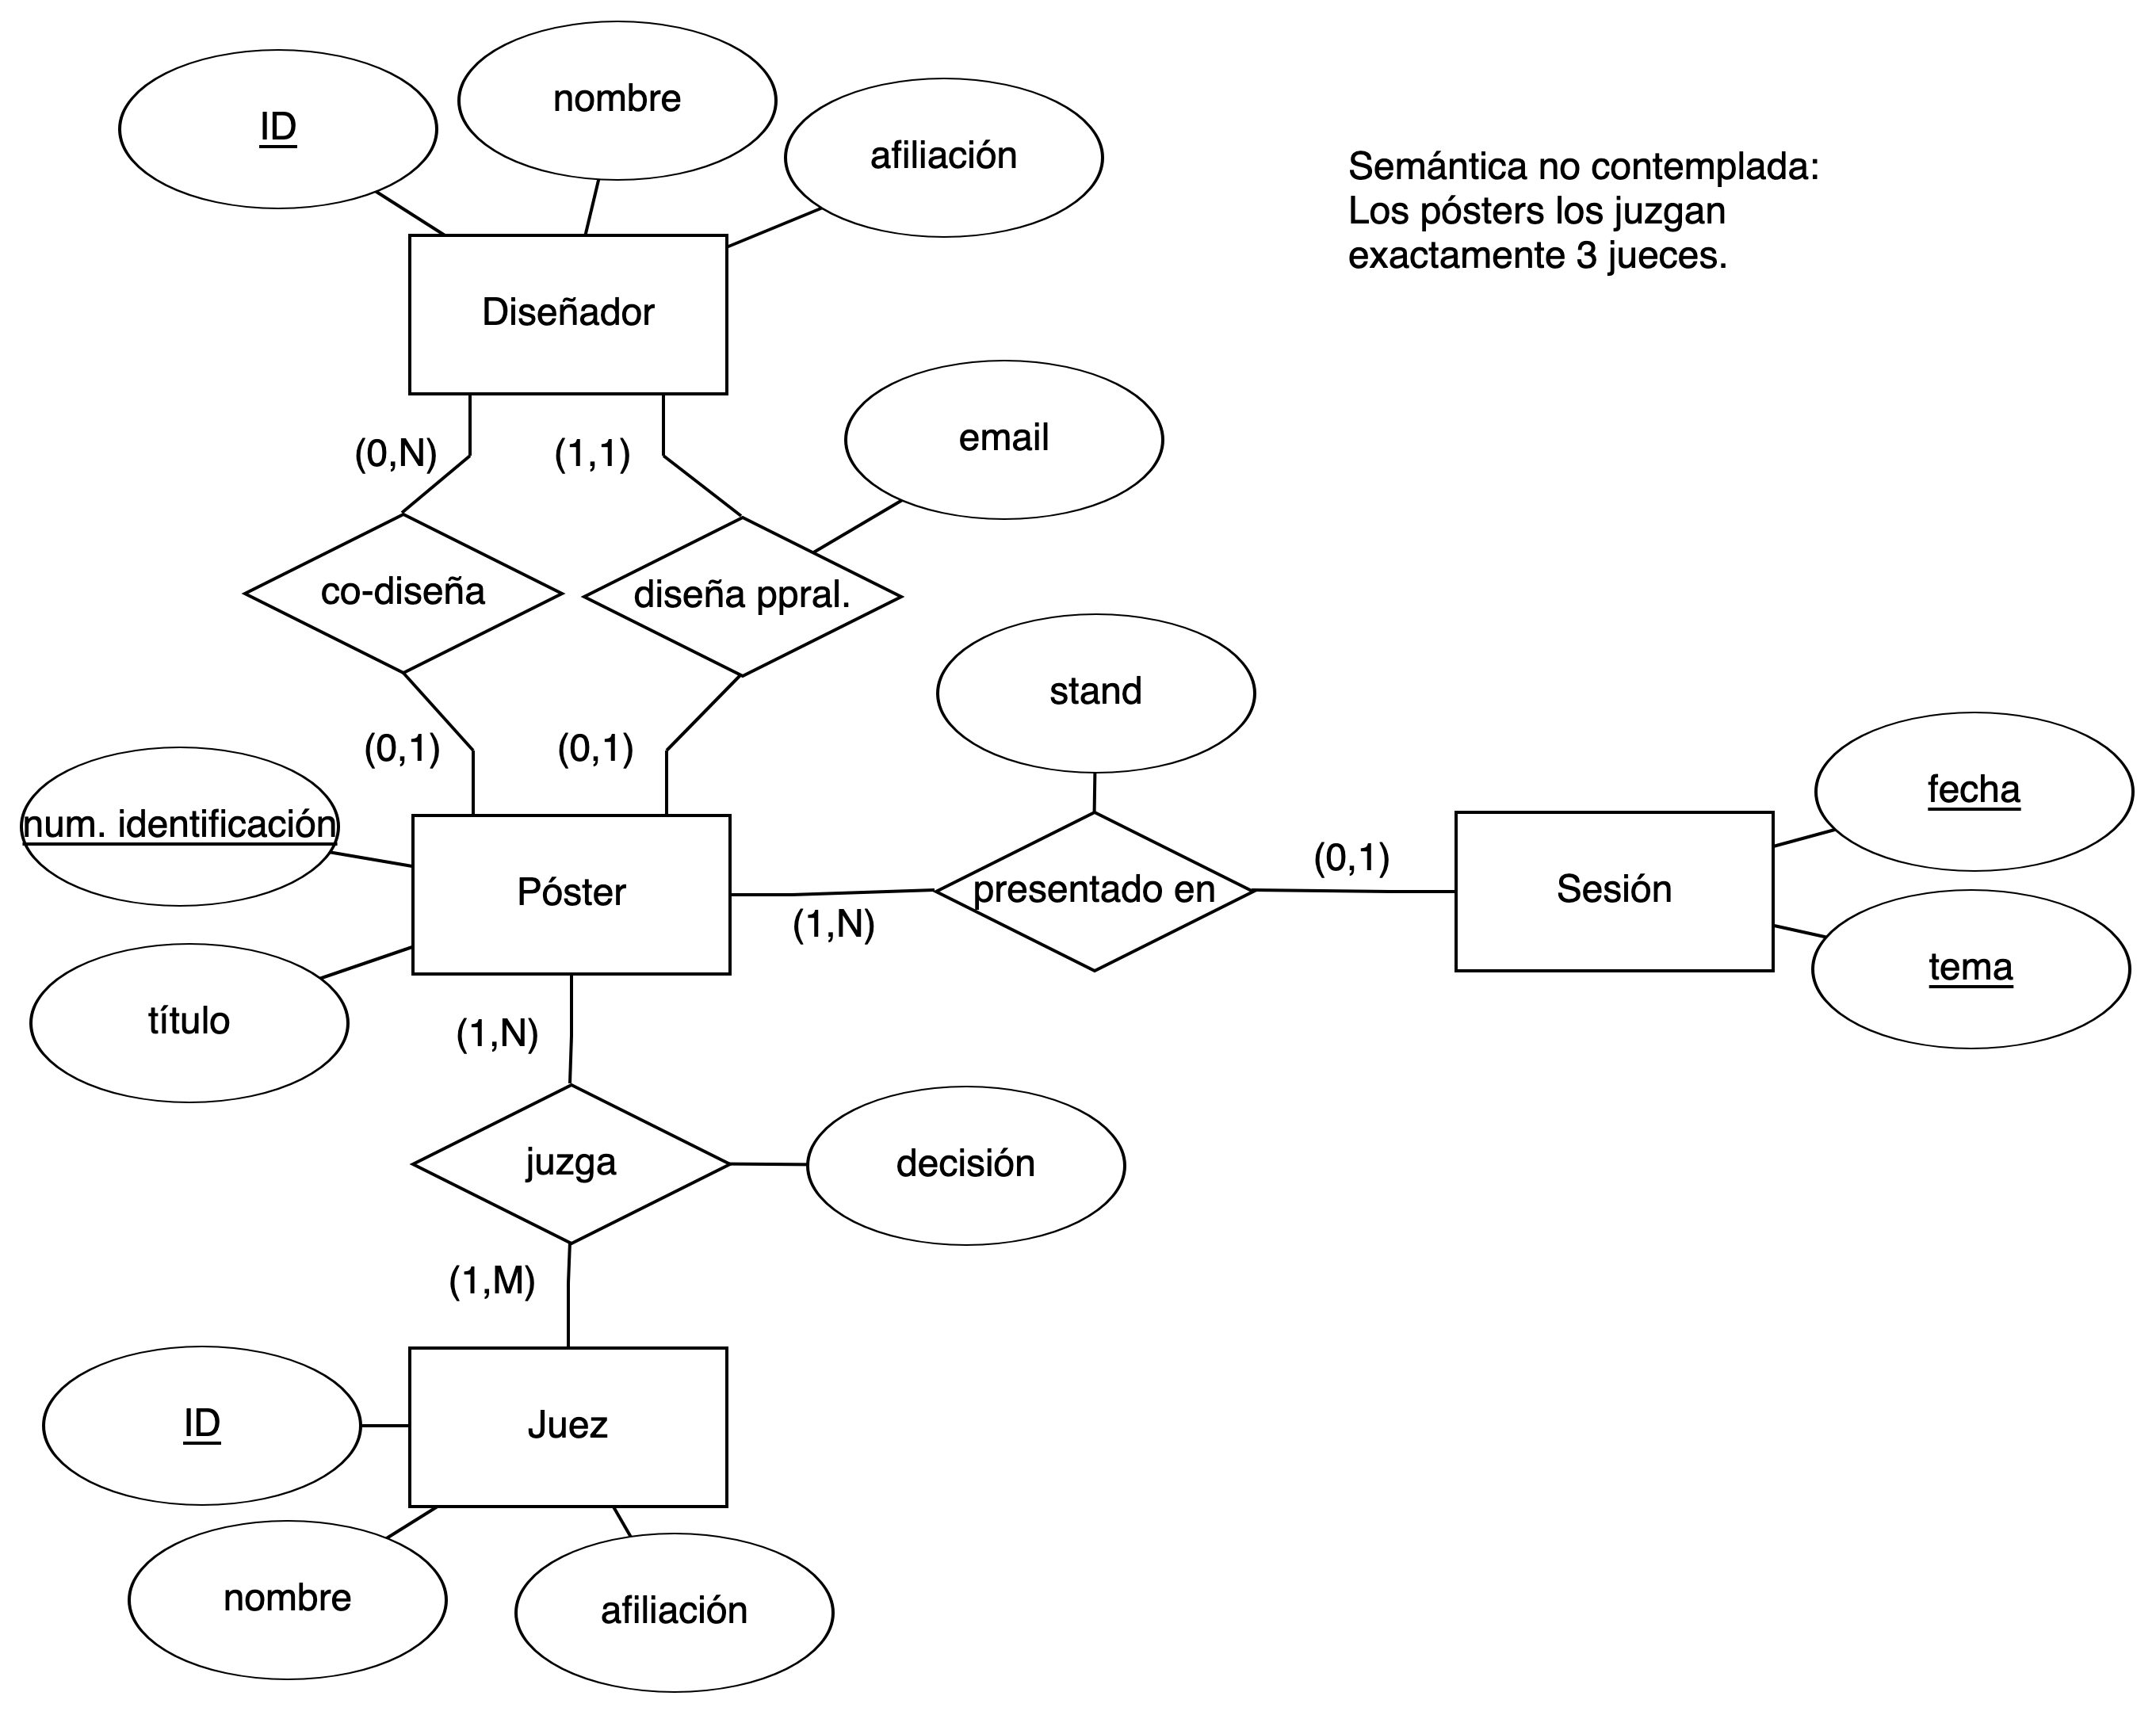
\includegraphics[width=\textwidth]{figs/ejercicio-12}
\end{figure}

\section{Desarrollo dirigidos por modelos}
\begin{figure}[H]
    \centering
    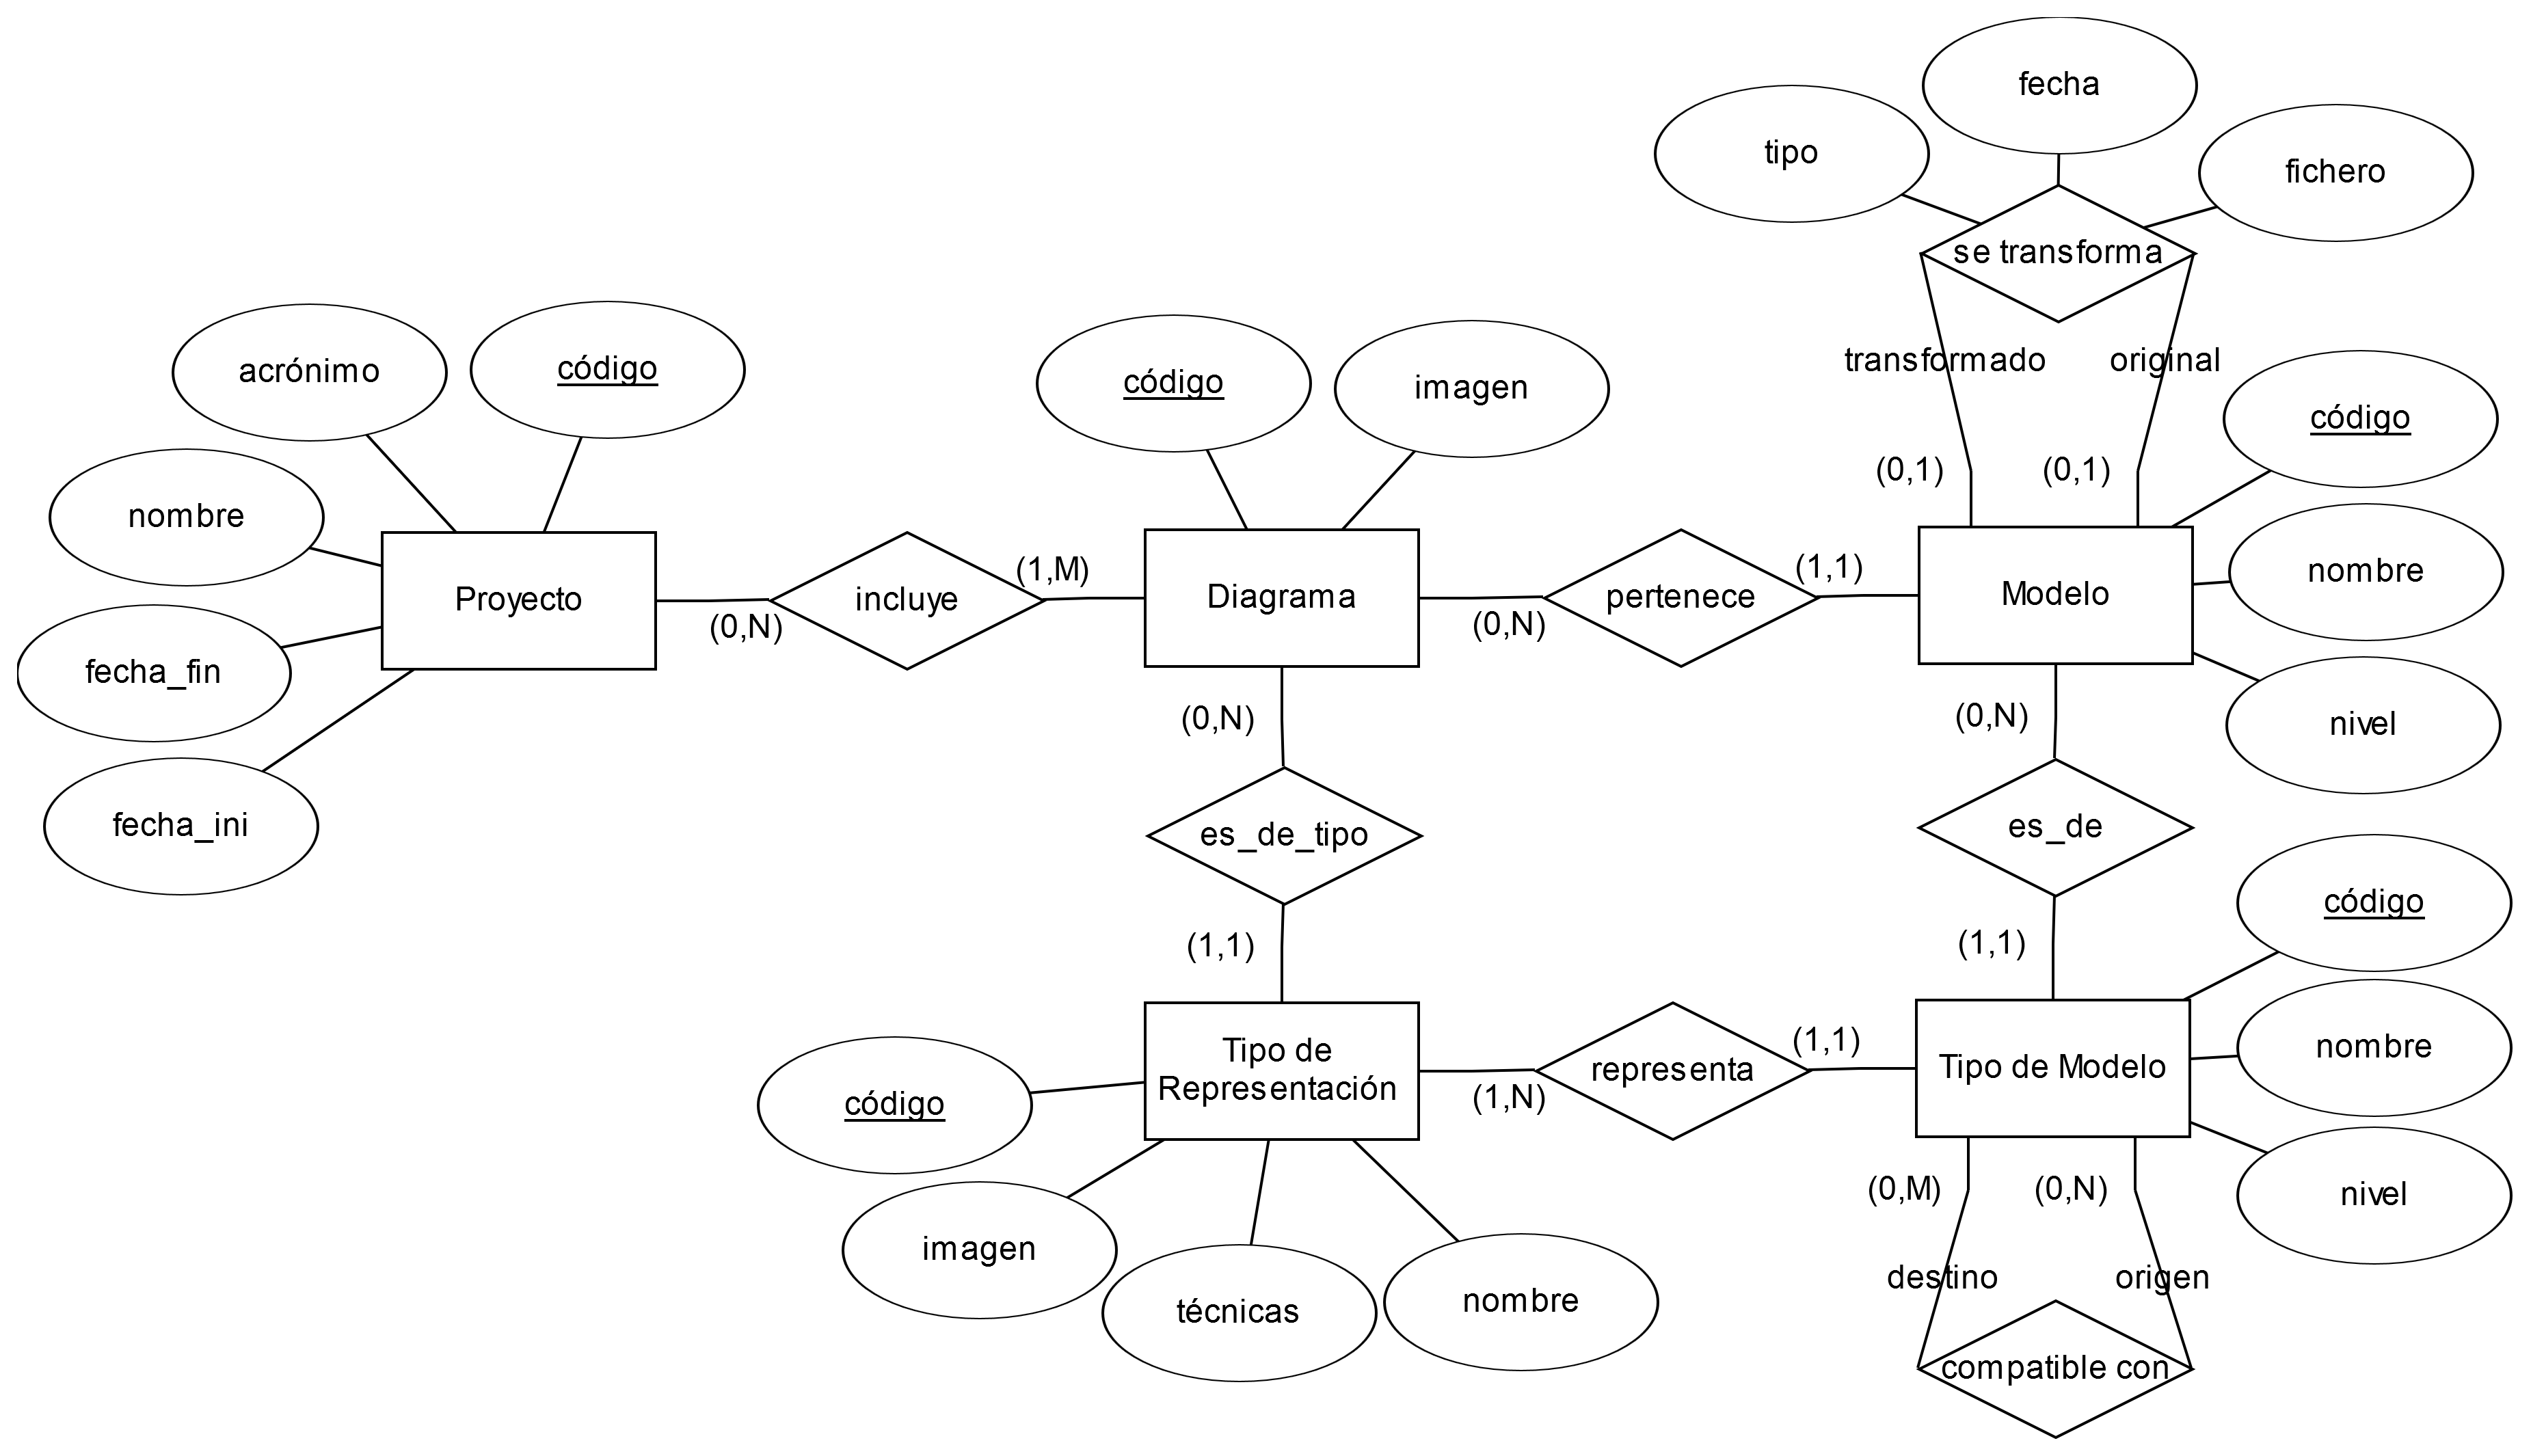
\includegraphics[width=\textwidth]{figs/ejercicio-13}
\end{figure}

\section{Gestión de locales nocturnos}
\begin{figure}[H]
    \centering
    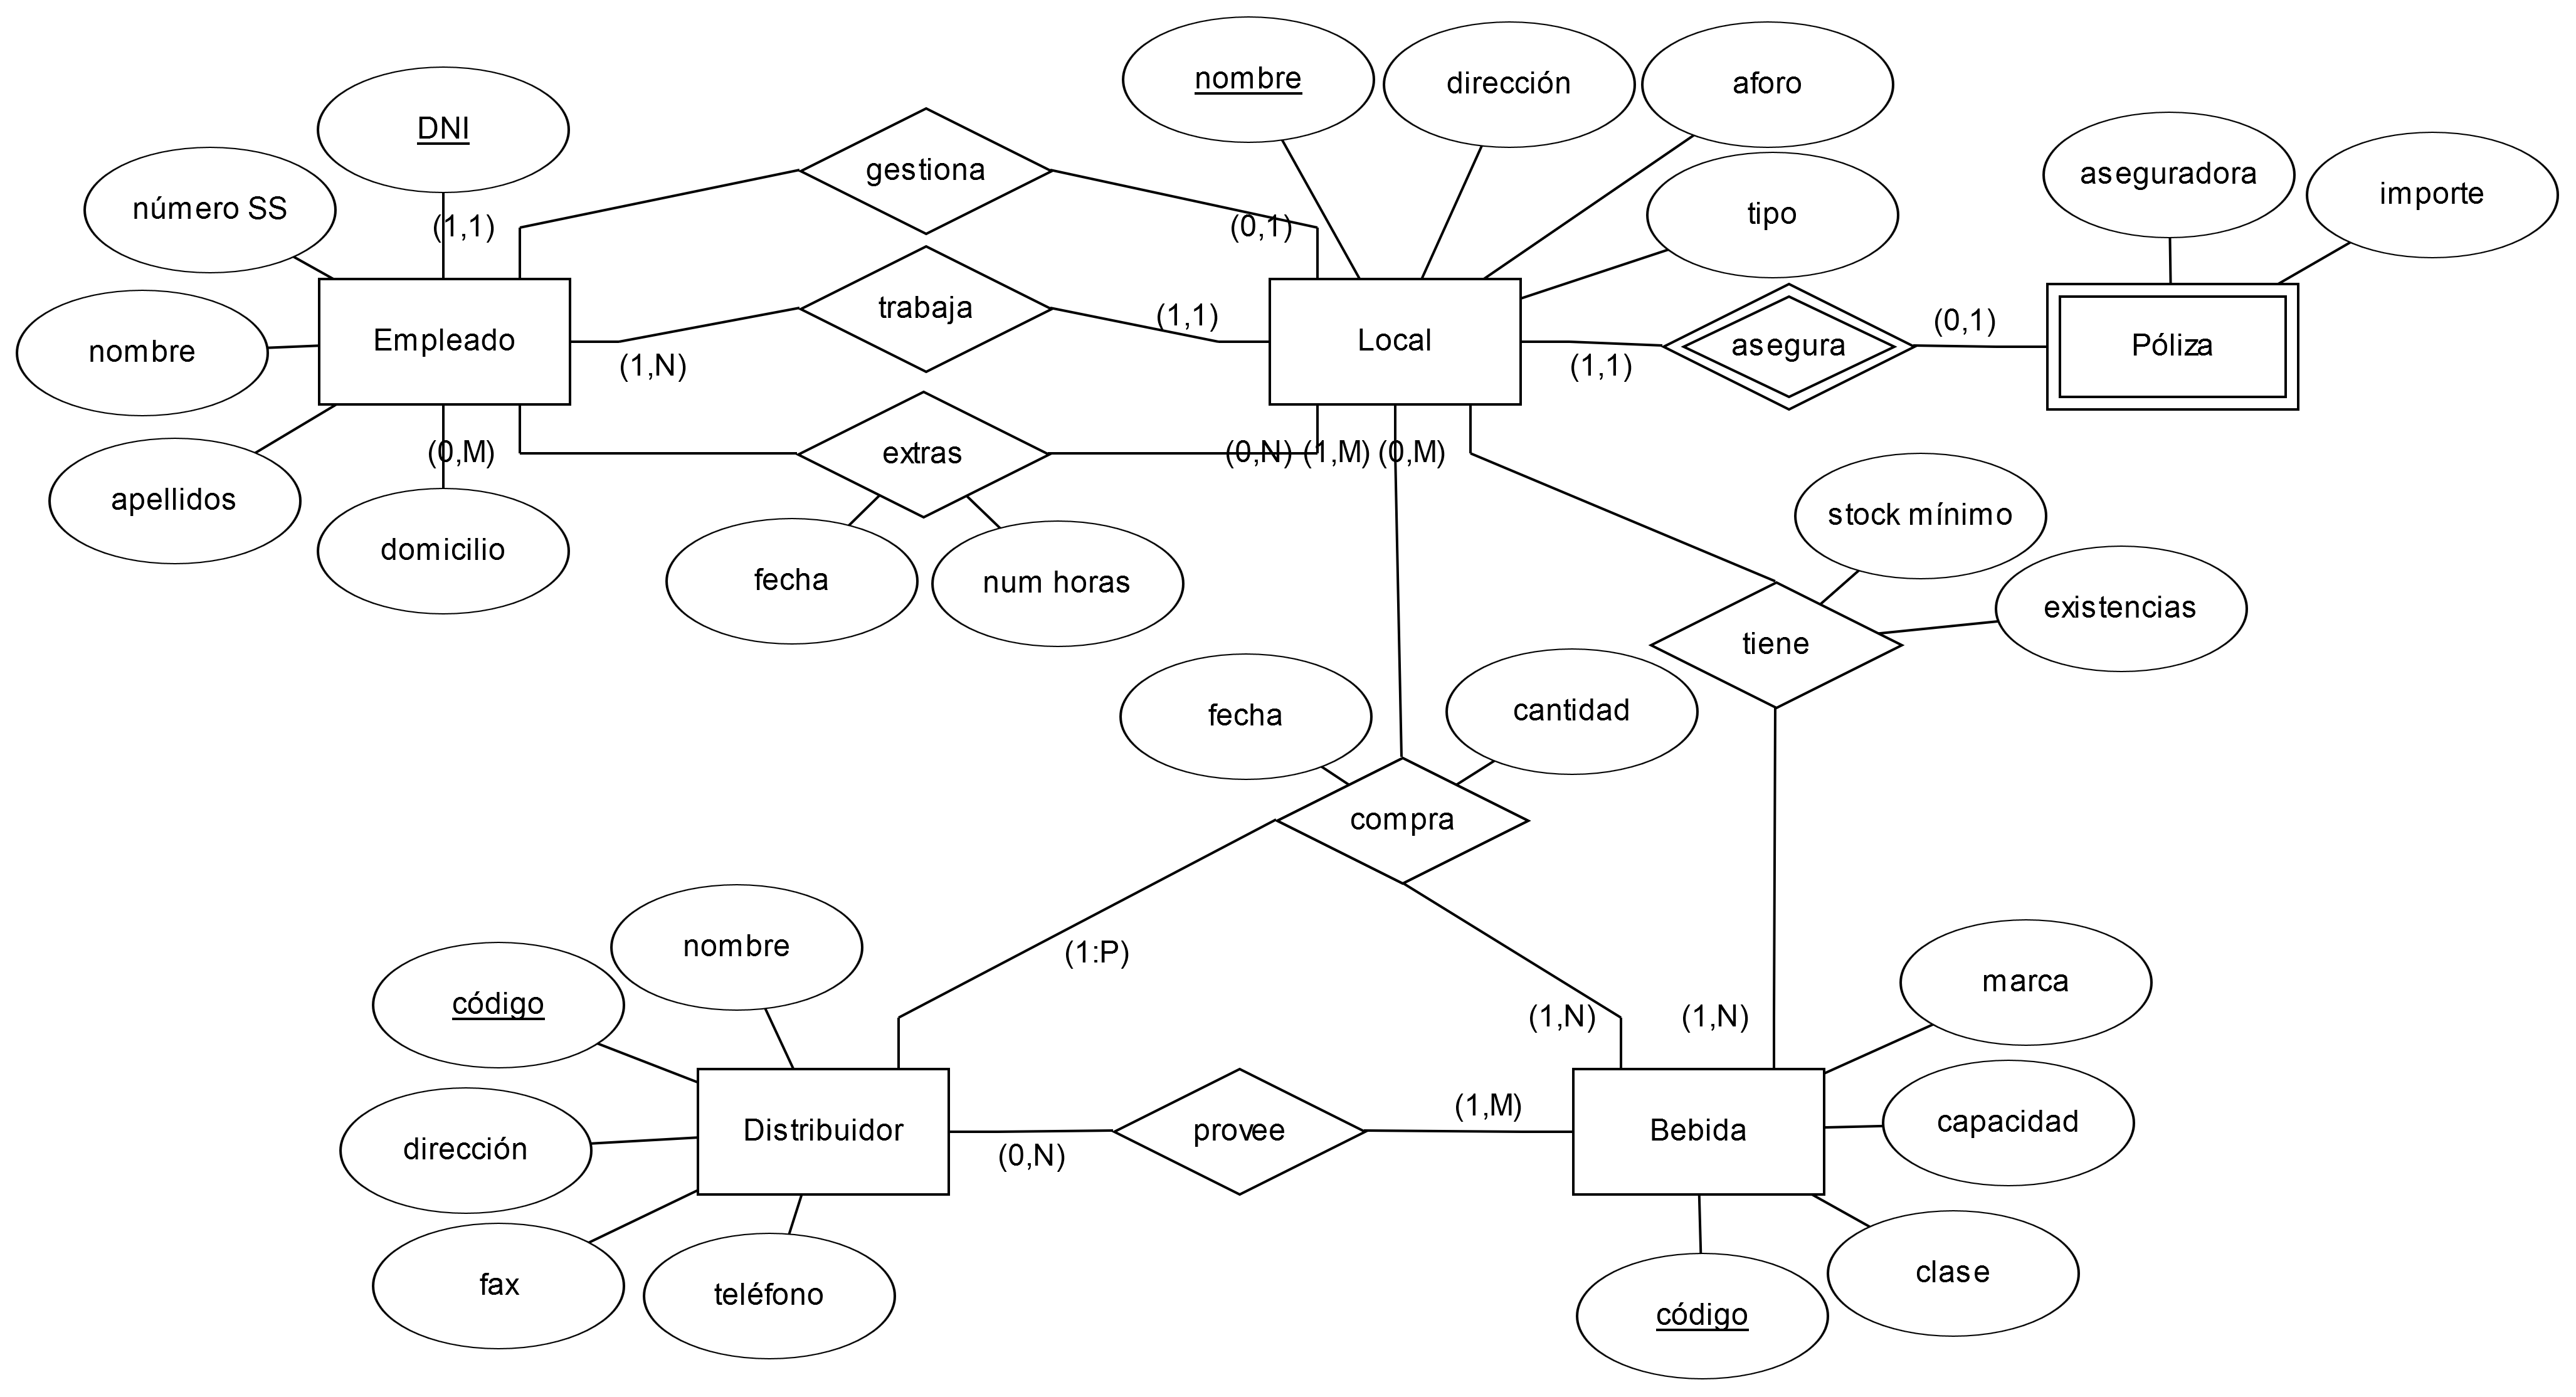
\includegraphics[width=\textwidth]{figs/ejercicio-14}
\end{figure}

\section{Empresa de telefonía}
\begin{figure}[H]
    \centering
    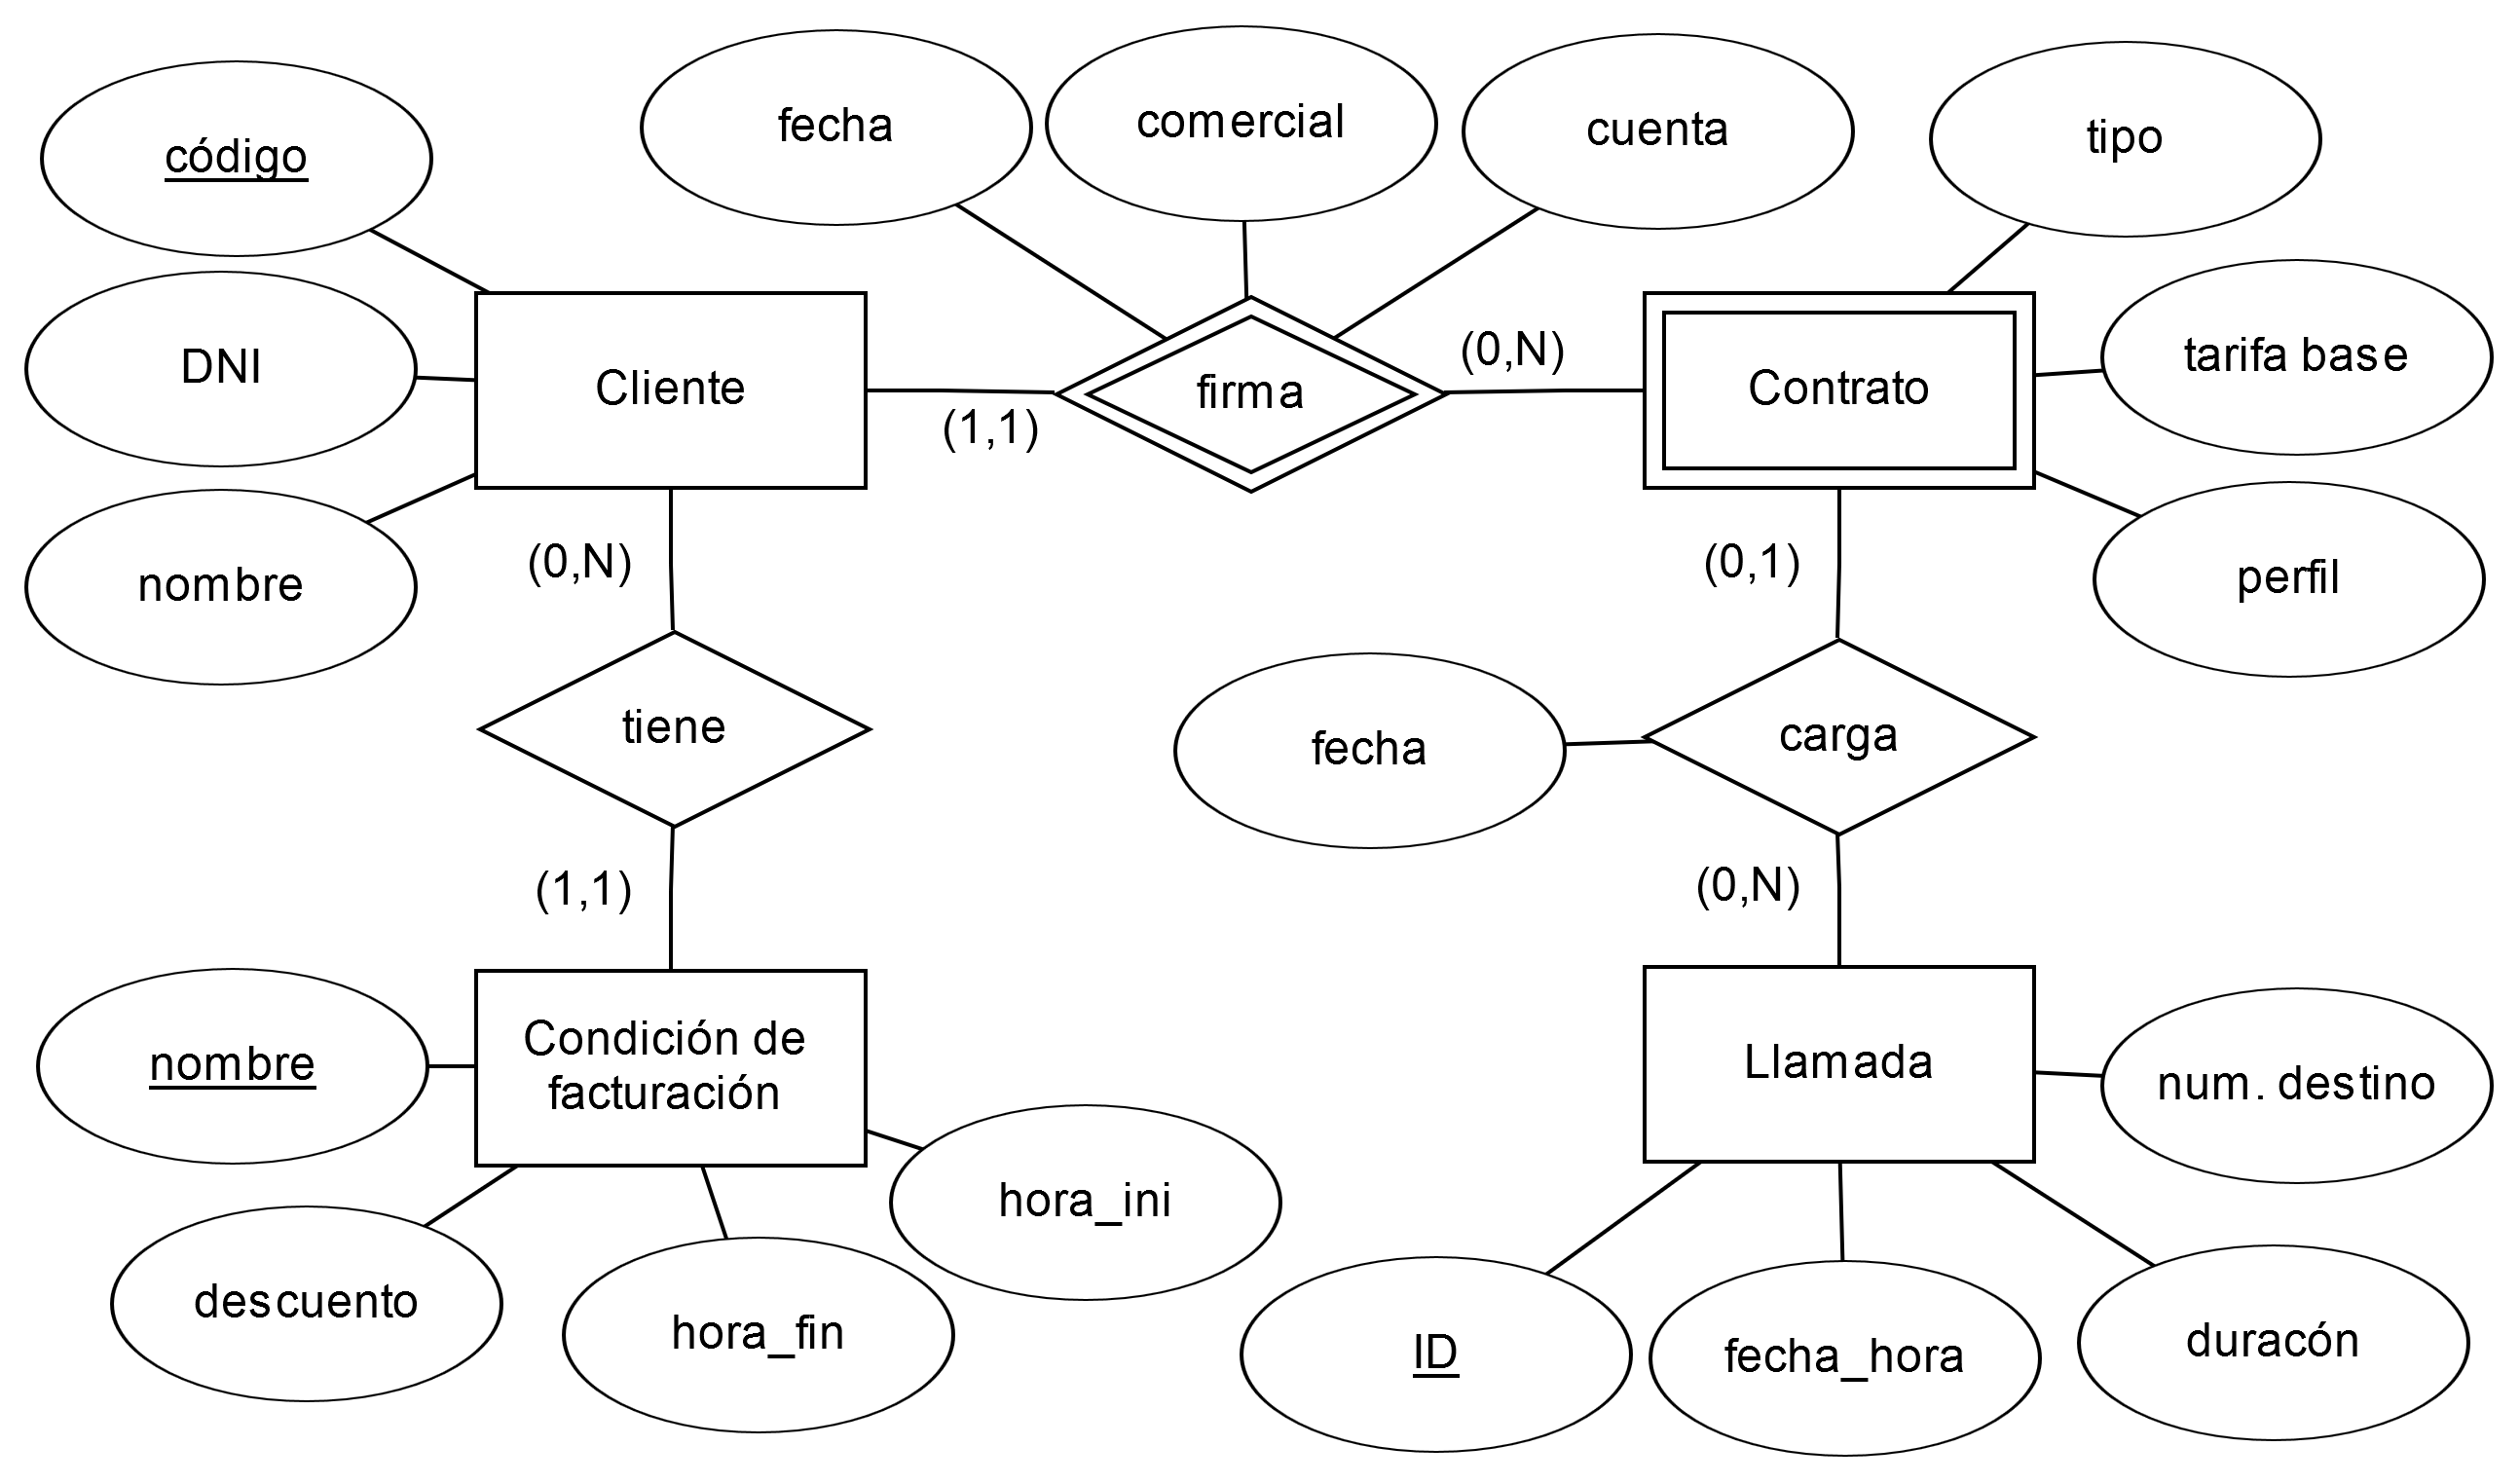
\includegraphics[width=\textwidth]{figs/ejercicio-15}
\end{figure}

\section{Gestión de proyectos y comercial}
\begin{figure}[H]
    \centering
    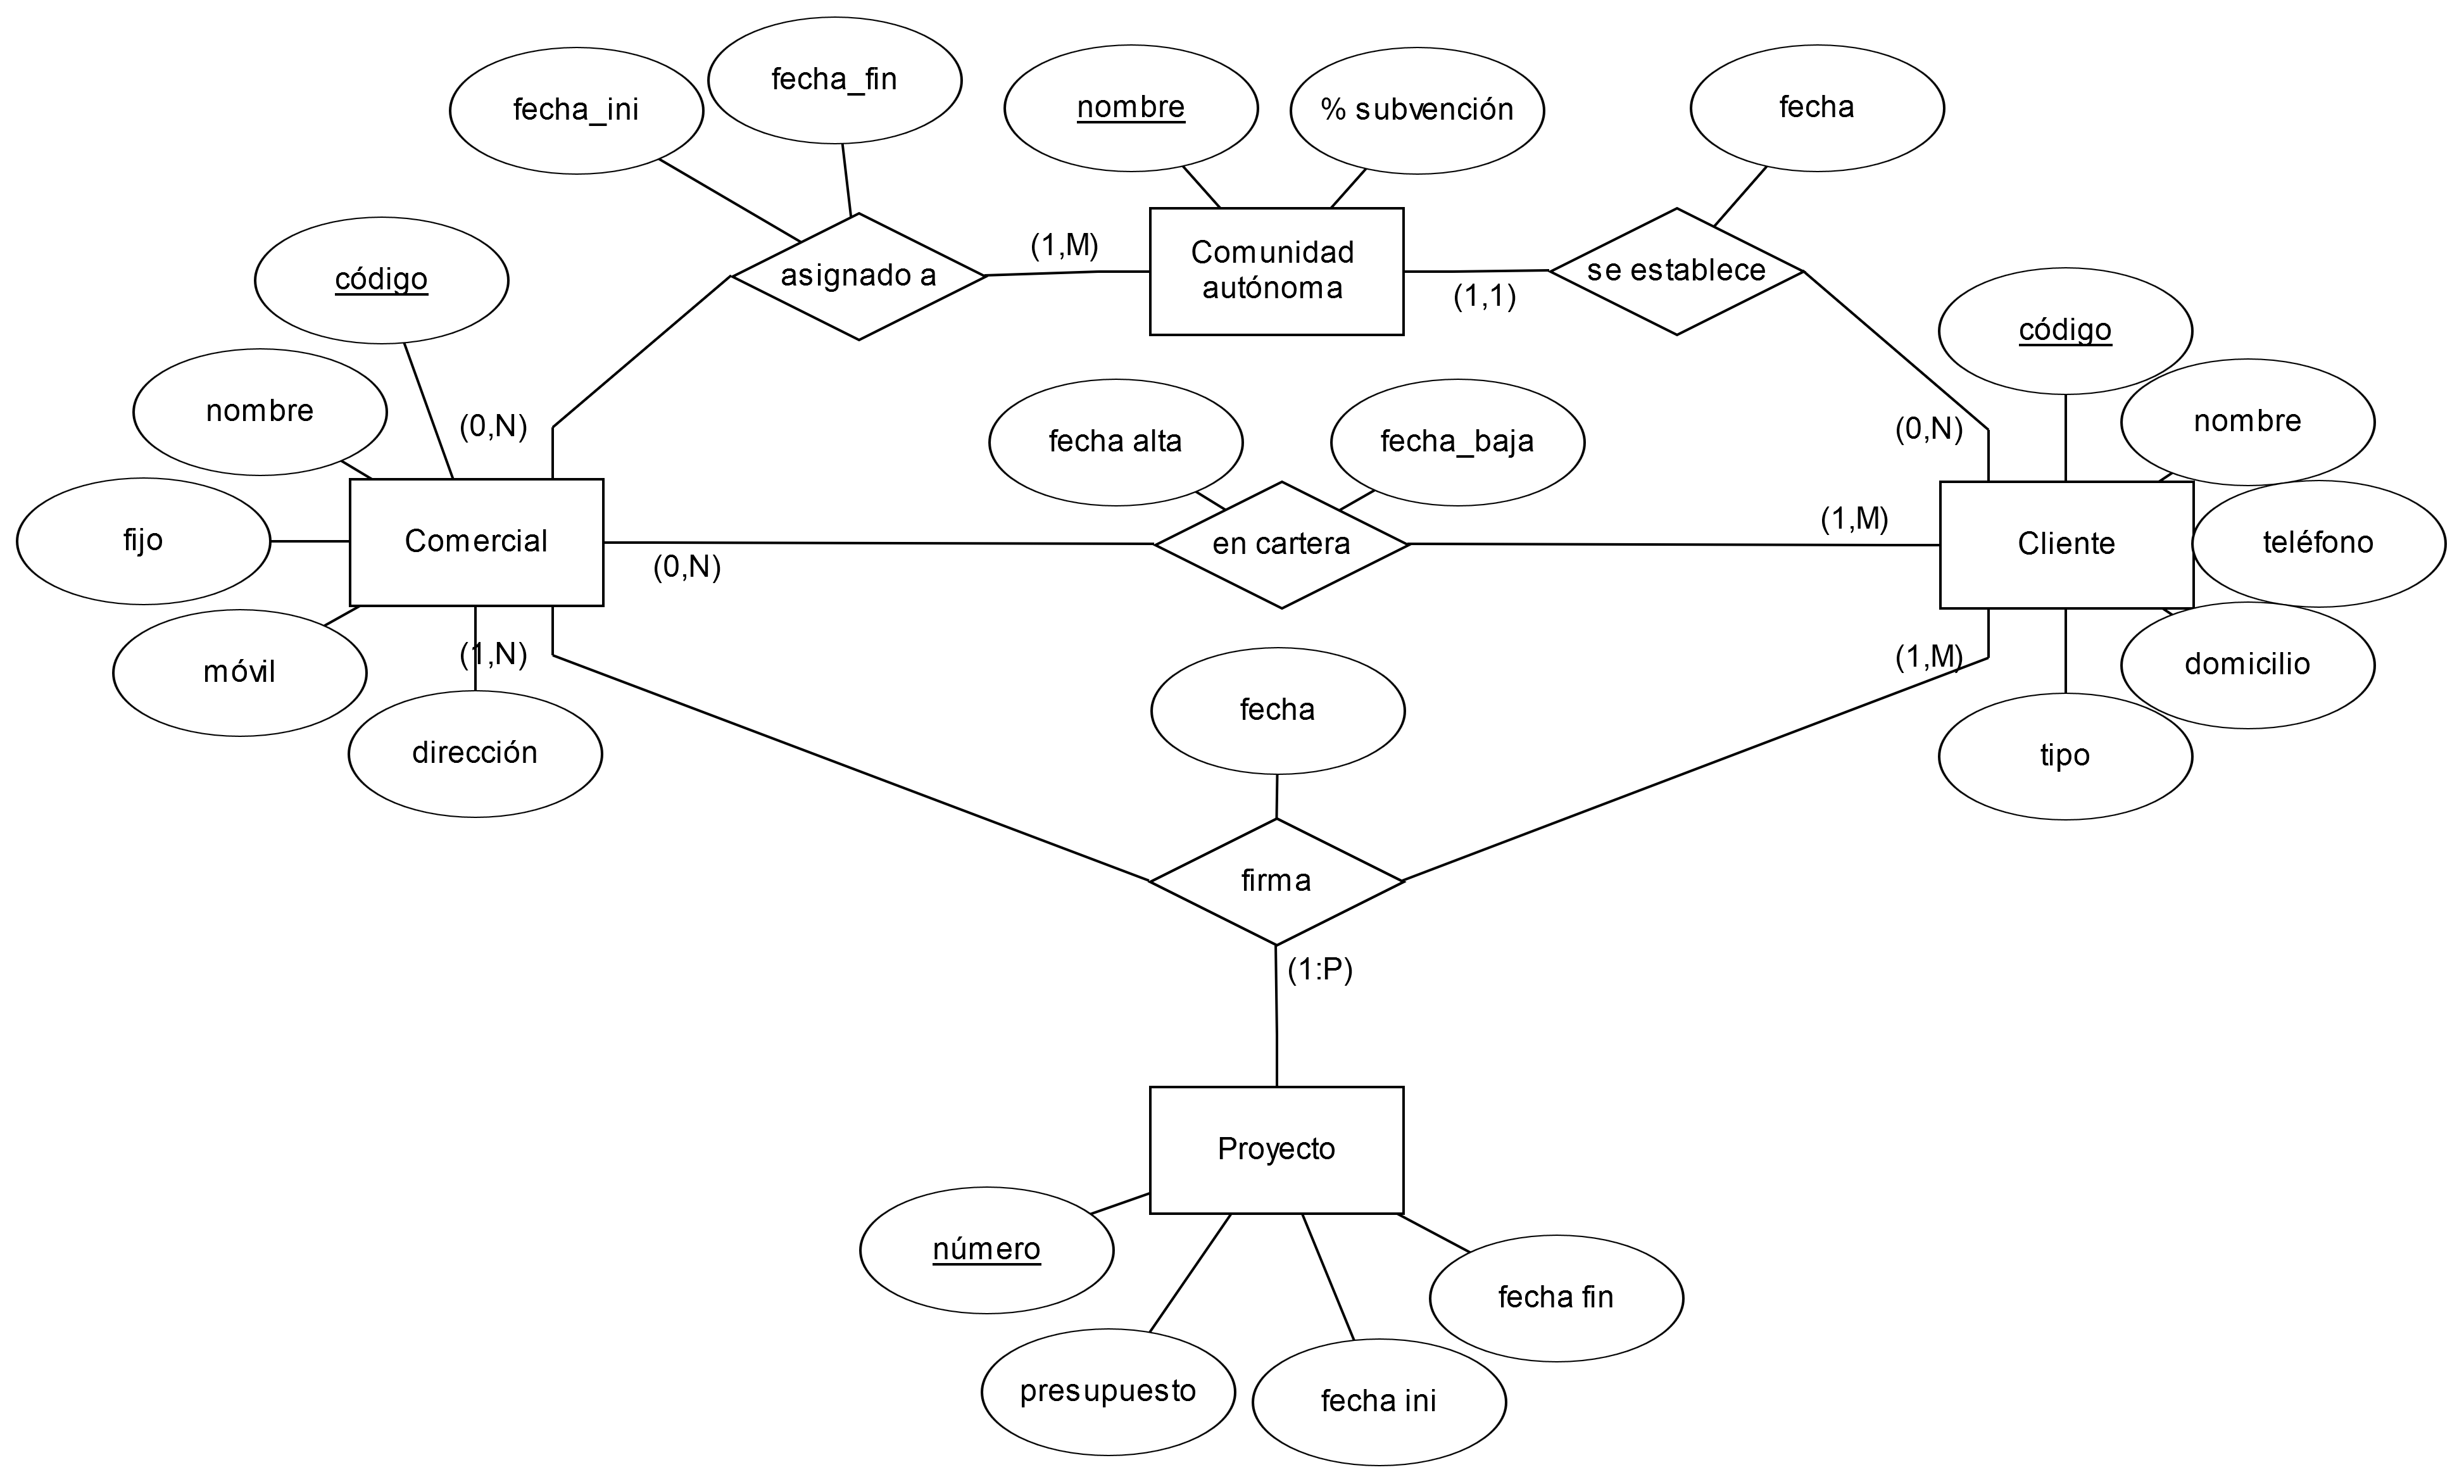
\includegraphics[width=\textwidth]{figs/ejercicio-16}
\end{figure}

\section{Puerto comercial}
\begin{figure}[H]
    \centering
    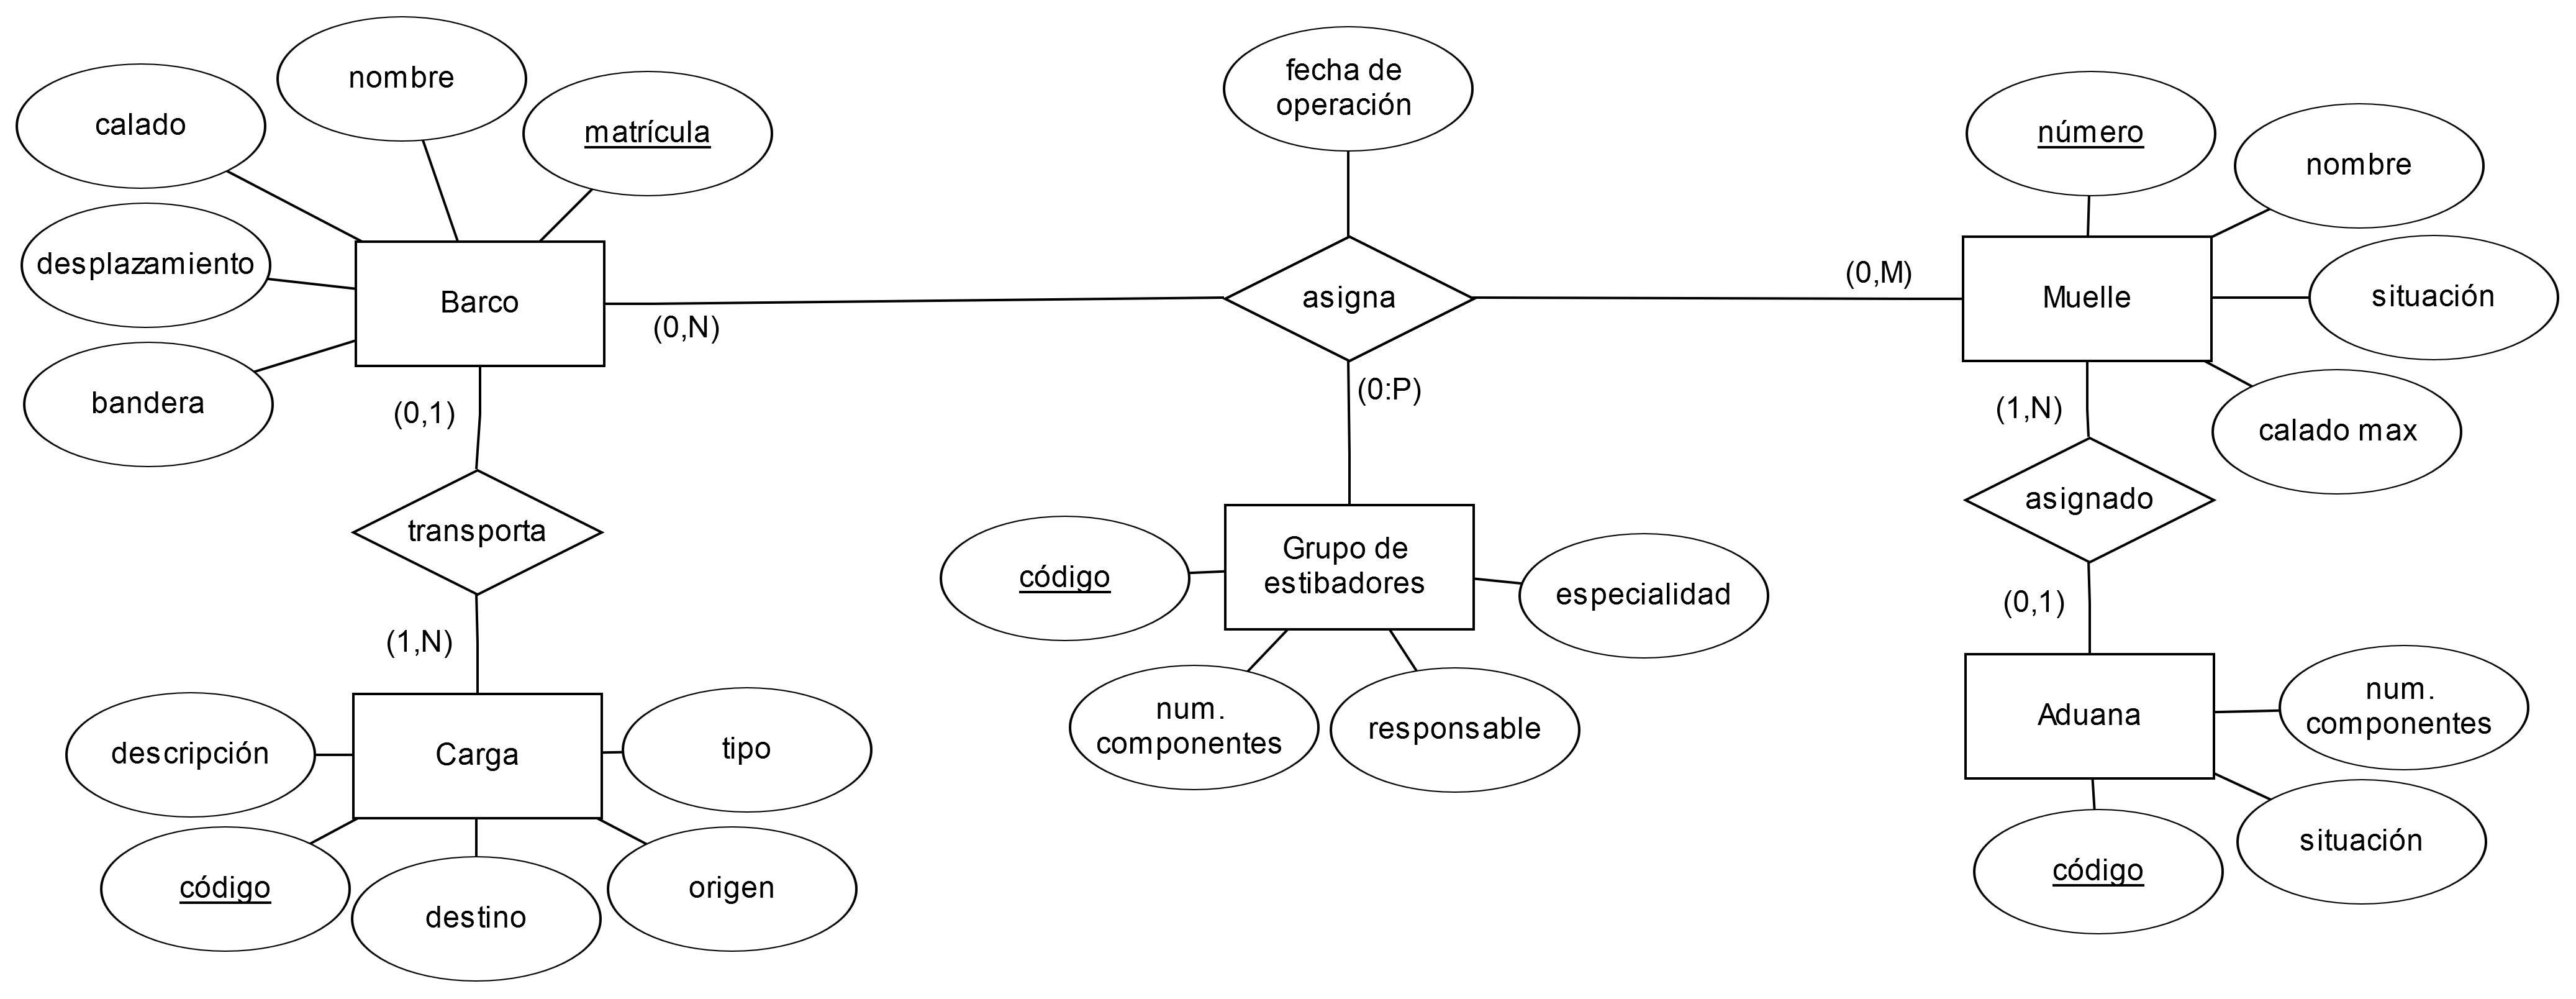
\includegraphics[width=\textwidth]{figs/ejercicio-17}
\end{figure}

\vspace{2em}
\hrule
\doclicenseThis

\end{document}
